%  LaTeX support: latex@mdpi.com
%  For support, please attach all files needed for compiling as well as the log file, and specify your operating system, LaTeX version, and LaTeX editor.

%=================================================================
\documentclass[remotesensing,article,submit,moreauthors,pdftex]{Definitions/mdpi}

% For posting an early version of this manuscript as a preprint, you may use "preprints" as the journal and change "submit" to "accept". The document class line would be, e.g., \documentclass[preprints,article,accept,moreauthors,pdftex]{mdpi}. This is especially recommended for submission to arXiv, where line numbers should be removed before posting. For preprints.org, the editorial staff will make this change immediately prior to posting.

%--------------------
% Class Options:
%--------------------

%----------
% submit
%----------
% The class option "submit" will be changed to "accept" by the Editorial Office when the paper is accepted. This will only make changes to the frontpage (e.g., the logo of the journal will get visible), the headings, and the copyright information. Also, line numbering will be removed. Journal info and pagination for accepted papers will also be assigned by the Editorial Office.

%------------------
% moreauthors
%------------------
% If there is only one author the class option oneauthor should be used. Otherwise use the class option moreauthors.

%=================================================================
% MDPI internal commands
\firstpage{1}
\makeatletter
\setcounter{page}{\@firstpage}
\makeatother
\pubvolume{1}
\issuenum{1}
\articlenumber{0}
\pubyear{2021}
\copyrightyear{2020}
%\externaleditor{Academic Editor: Firstname Lastname} % For journal Automation, please change Academic Editor to "Communicated by"
\datereceived{}
\dateaccepted{}
\datepublished{}
\hreflink{https://doi.org/} % If needed use \linebreak
%------------------------------------------------------------------
% The following line should be uncommented if the LaTeX file is uploaded to arXiv.org
%\pdfoutput=1

%=================================================================
% Add packages and commands here. The following packages are loaded in our class file: fontenc, inputenc, calc, indentfirst, fancyhdr, graphicx, epstopdf, lastpage, ifthen, lineno, float, amsmath, setspace, enumitem, mathpazo, booktabs, titlesec, etoolbox, tabto, xcolor, soul, multirow, microtype, tikz, totcount, changepage, paracol, attrib, upgreek, cleveref, amsthm, hyphenat, natbib, hyperref, footmisc, url, geometry, newfloat, caption

% \usepackage[noadjust]{cite}
% \usepackage[hidelinks]{hyperref}
\usepackage[nolist]{acronym}

\usepackage{tabularx}
\usepackage{booktabs}
\usepackage{multirow}
\usepackage{adjustbox}

% \usepackage{supertabular}
\usepackage{supertabular,booktabs}

% line breaks in table cells
\newcommand{\specialcell}[2][l]{%
  \begin{tabular}[#1]{@{}l@{}}#2\end{tabular}}

\usepackage{csquotes}
\usepackage[utf8]{inputenc}
% enables custom font styles which are not available in IEEEtran by default
% https://tex.stackexchange.com/questions/331228/there-is-no-bold-text-italics-in-ieeetran

\renewcommand{\sfdefault}{cmss}
\renewcommand{\rmdefault}{cmr}
\renewcommand{\ttdefault}{cmt}

\usepackage[detect-all]{siunitx}

\usepackage[pdftex]{graphicx}
% declare the path(s) where your graphic files are
\graphicspath{{./pdf/}{./jpg/}}
% and their extensions so you won't have to specify these with
% every instance of \includegraphics
\DeclareGraphicsExtensions{.pdf,.jpg,.png}

% suppress fancyhdr warnings
\setlength{\headheight}{23.90979pt}

% *** MATH PACKAGES ***
%
\usepackage{amsmath}
\newcommand*\mean[1]{\bar{#1}}

%=================================================================
%% Please use the following mathematics environments: Theorem, Lemma, Corollary, Proposition, Characterization, Property, Problem, Example, ExamplesandDefinitions, Hypothesis, Remark, Definition, Notation, Assumption
%% For proofs, please use the proof environment (the amsthm package is loaded by the MDPI class).

%=================================================================
% Full title of the paper (Capitalized)
\Title{Monitoring forest health using hyperspectral imagery: Does feature selection improve the performance of machine-learning techniques?}

% MDPI internal command: Title for citation in the left column
\TitleCitation{Title}

% Author Orchid ID: enter ID or remove command
\newcommand{\orcidauthorA}{0000-0003-0748-6624} % Add \orcidA{} behind the author's name
\newcommand{\orcidauthorB}{0000-0001-7834-4717} % Add \orcidB{} behind the author's name
\newcommand{\orcidauthorC}{0000-0003-2567-8689} % Add \orcidB{} behind the author's name
\newcommand{\orcidauthorD}{0000-0002-6390-5873} % Add \orcidB{} behind the author's name
\newcommand{\orcidauthorE}{0000-0001-6002-6980} % Add \orcidB{} behind the author's name
\newcommand{\orcidauthorF}{0000-0001-6640-679X} % Add \orcidB{} behind the author's name

% Authors, for the paper (add full first names)
\Author{Patrick Schratz $^{1}$\orcidA{}*, Jannes Muenchow $^{1}$\orcidB{}, Eugenia Iturritxa $^{2}$\orcidD{}, José Cortés $^{1}$\orcidC{}, Bernd Bischl $^{3}$\orcidE{} and Alexander Brenning $^{1,}$\orcidF{}}

% MDPI internal command: Authors, for metadata in PDF
\AuthorNames{Firstname Lastname, Firstname Lastname and Firstname Lastname}

% MDPI internal command: Authors, for citation in the left column
\AuthorCitation{Schratz, P.; Muenchow, J.; Cortés, J.; Iturritxa, E.; Bischl, B.; Brenning, A.}

% Affiliations / Addresses (Add [1] after \address if there is only one affiliation.)
\address{%
$^{1}$ \quad Friedrich Schiller University Jena, Department of Geography, GIScience group, Germany\\
$^{2}$ \quad NEIKER Tecnalia, Spain\\
$^{3}$ \quad Ludwig-Maximilians-Universität München, Department of Statistics, Computational Statistics group, Germany
}

% Contact information of the corresponding author
\corres{Correspondence: patrick.schratz@uni-jena.de}

% Current address and/or shared authorship
% \firstnote{Current address: Affiliation 3}
% \secondnote{These authors contributed equally to this work.}
% The commands \thirdnote{} till \eighthnote{} are available for further notes

%\simplesumm{} % Simple summary

% Abstract (Do not insert blank lines, i.e. \\)
\abstract{This study analyzed highly correlated, feature-rich datasets from hyperspectral remote sensing data using multiple statistical and machine-learning methods.
The effect of filter-based feature selection methods on predictive performance was compared.
Also, the effect of multiple expert-based and data-driven feature sets, derived from the reflectance data, was investigated.
Defoliation of trees (\%), derived from in-situ measurements from fall 2016, was modeled as a function of reflectance.
Variable importance was assessed using permutation-based feature importance.
Overall, the support vector machine (SVM) outperformed other algorithms such as random forest (RF), extreme gradient boosting (XGBoost), and lasso (L1) and ridge (L2) regressions by at least three percentage points.
The combination of certain feature sets showed small increases in predictive performance while no substantial differences between individual feature sets were observed.
For some combinations of learners and feature sets, filter methods achieved better predictive performances than using no feature selection.
Ensemble filters did not have a substantial impact on performance.
The most important features were located around the red edge.
Additional features in the near-infrared region (800 nm - 1000 nm) were also essential to achieve the overall best performances.
Filter methods have the potential to be helpful in high-dimensional situations and are able to improve the interpretation of feature effects in fitted models, which is an essential constraint in environmental modeling studies.
Nevertheless, more training data and replication in similar benchmarking studies are needed to be able to generalize the results.}

% Keywords
\keyword{hyperspectral imagery; forest health monitoring; machine learning; feature selection; model comparison}

% The fields PACS, MSC, and JEL may be left empty or commented out if not applicable
%\PACS{J0101}
%\MSC{}
%\JEL{}

\begin{acronym}

	% geringerer Zeilenabstand

	%\setlength{\itemsep}{-\parsep}
	\acro{AGB}{above-ground biomass}
	\acro{ALE}{accumulated local effects}
	\acro{ALS}{airborne laser scanning}
	\acro{ANN}{artificial neural network}
	\acro{AUROC}{area under the receiver operating characteristics curve}
	\acro{BRT}{boosted regression trees}
	\acro{CART}{classification and regression trees}
	\acro{CNN}{convolutional neural networks}
	\acro{CV}{cross-validation}
	\acro{DAP}{digital aerial photogrammetry}
	\acro{ENM}{environmental niche modeling}
	\acro{FFS}{forward feature selection}
	\acro{FPR}{false-positive rate}
	\acro{FS}{feature selection}
	\acro{GAM}{generalized additive model}
	\acro{GBM}{gradient boosting machine}
	\acro{GLM}{generalized linear model}
	\acro{ICGC}{Institut Cartografic i Geologic de Catalunya}
	\acro{IQR}{interquartile range}
	\acro{LiDAR}{light detection and ranging}
	\acro{LOWESS}{locally weighted scatterplot smoothing}
	\acro{MARS}{multivariate adaptive regression splines}
	\acro{MBO}{model-based optimization}
	\acro{MEM}{maximum entropy model}
	\acro{ML}{machine learning}
	\acro{NDII}{normalized difference infrared index}
	\acro{NDMI}{normalized difference moisture index}
	\acro{NIR}{near-infrared}
	\acro{NRI}{normalized ratio index}
	\acro{OLS}{ordinary least squares}
	\acro{OMNBR}{optimized multiple narrow-band reflectance}
	\acro{PCA}{principal component analysis}
	\acro{PDP}{partial dependence plots}
	\acro{PISR}{potential incoming solar radiation}
	\acro{PLS}{partial least squares}
	\acro{POV}{proportion of variance explained}
	\acro{RBF}{radial basis function}
	\acro{RF}{random forest}
	\acro{RMSE}{root mean square error}
	\acro{RR}{ridge regression}
	\acro{RSS}{residual sum of squares}
	\acro{SAR}{synthetic aperture radar}
	\acro{SDM}{species distribution modeling}
	\acro{SMBO}{sequential model-based optimization}
	\acro{SVM}{support vector machine}
	\acro{TPR}{true-positive rate}
	\acro{VI}{vegetation index}
	\acro{XGBoost}{extreme gradient boosting}
	\acro{PC}{principal component}
\end{acronym}

\begin{document}
\section{Introduction}

The use of \ac{ML} algorithms for analyzing remote sensing data has seen a huge increase in the last decade \cite{lary2016}.
This coincided with the increased availability of remote sensing imagery, especially since the launch of the first Sentinel satellite in the year 2014.
At the same time, the implementation and usability of learning algorithms has been greatly simplified with many contributions from the open-source community.
Scientists can nowadays process large amounts of (environmental) information with relative ease using various learning algorithms.
This makes it possible to easily extend benchmark comparison matrices of studies in a semi-automated way, possibly stumbling upon unexpected findings such as process settings that would not have been explored otherwise \cite{ma2015}.

% link to forest health (defoliation) analysis and show exemplary studies

ML methods in combination with remote sensing data are used in many environmental fields such as vegetation cover analysis or forest carbon storage mapping \cite{mascaro2014, urban2018}.
The ability to predict these environmental variables in unknown regions qualifies ML algorithms as a helpful tool for such environmental analyses.
One aspect of this research field is to enhance the understanding of biotic and abiotic stress triggers, for example by analyzing tree defoliation \cite{hawrylo2018}.
Defoliation is known to be a proxy for pathogen and insect damage \cite{pollastrini2016}.
While common symptoms are observable across species, some effects and their degree of severity are species-specific \cite{gottardini2020}.
Defoliation has also been shown to increase predisposition of tree death from secondary biotic factors up to ten years after the actual defoliation event \cite{oliva2016}.
Other approaches for analyzing forest health include change detection \cite{zhang2016}, or describing the current health status of forests on a stand level \cite{townsend2012}.

% introduce veg indices
Vegetation indices have shown the potential to provide valuable information when analyzing forest health \cite{jiang2014, adamczyk2015}.
Most vegetation indices were developed with the aim of being sensitive to changes in specific wavelength regions, serving proxies for underlying plant physiological processes.
In some cases, indices developed for different purposes than the one to be analyzed (e.g., defoliation of pine trees) may help to explain complex underlying relationships that are not obvious at first.
This emphasizes the need to extract as much information as possible from the available input data to generate promising features which can help to understand the modeled relationship \cite{thenkabail2018}.
A less known index type that can be derived from spectral information is the \ac{NRI}.
In contrast to most vegetation indices, \ac{NRI}s do not use an expert-based formula following environmental heuristics; instead, they make use of a data-driven feature engineering approach by combining (all possible) combinations of spectral bands \cite{thenkabail2000}.
When working with hyperspectral data, thousands of \ac{NRI} features can be derived this way.

% mention why FS is used / important
Even though \ac{ML} algorithms are capable of handling highly correlated input variables, model fitting becomes computationally more demanding, and model interpretation more challenging.
Feature selection approaches can help to address this issue, reducing possible noise in the feature space, simplifing model interpretability, and possibly enhancing predictive performance \cite{cai2018}.
Instead of using wrapper feature selection methods, which add a substantial overhead to a nested model optimization approach, especially for datasets with many features, this study focuses on (ensemble) filter methods, which can be directly integrated into the hyperparameter optimization step during model construction.

% clarify the focus of this study
Overall, this study aims to show how high-dimensional datasets can be handled effectively with ML methods while still allowing the interpretation of the fitted models.
The predictive power of non-linear methods and their ability to handle highly correlated predictors is combined with common and new approaches for assessing feature importance and feature effects.
Yet, this study focuses mainly on investigating the effects of filter methods and feature set types on predictive performance rather than interpreting individual feature effects.

Considering these opportunities and challenges, the research questions of this study are the following:

\begin{itemize}

	\item How do different feature selection methods influence the predictive performance of ML models of the defoliation of trees?

	\item Do different (environmental) feature sets show differences in performance?

	\item Can predictive performance be substantially improved by combining feature sets?

	\item Which features are most important and how can these be interpreted in this context?

\end{itemize}

% Explain what is new in this study and link to methodology
In recent years, various studies that have used hyperspectral data to analyze pest/fungi infections on trees have been published:
Pinto et al. \citep{pinto2020} successfully used hyperspectral imagery to characterize pest infections on peanut leaves using random forest while Yu et. al \cite{yu2021} aimed to detect pine wilt disease in pine plots in China using vegetation indices derived from hyperspectral data.
Other studies which applied hyperspectral data for forest health monitoring are \cite{lin2014,kayet2019,dash2017}.
Building upon these successful applications of hyperspectral remote sensing usage in the field of leaf and tree health monitoring, this work analyses tree defoliation in northern Spain using airborne hyperspectral data.
The methodology of this study uses ML methods in combination with feature selection and hyperparameter tuning.
In addition, feature importance was analyzed.
Incorporating the idea of creating data-driven \ac{NRI}s, this study also discusses the practical problems of high dimensionality in environmental modeling \cite{trunk1979, xu2016}.

%%%%%%%%%%%%%%%%%%%%%%%%%%%%%%%%%%%%%%%%%%
\section{Materials and Methods}

\subsection{Data and study area}

Airborne hyperspectral data with a spatial resolution of one meter and 126 spectral bands was available for four Monterey Pine (\textit{Pinus radiata D. Don}) plantations in northern Spain.
The trees in the plots suffer from infections with pathogens such as \textit{Diplodia sapinea (Fr.) Fuckel}, \textit{Fusarium circinatum Nirenberg \& O'Donnell}, \textit{Armillaria mellea (Vahl) P. Kumm}, \textit{Heterobasidion annosum (Fr.) Bref}, \textit{Lecanosticta acicola (Thüm) Syd.} and \textit{Dothisthroma septosporum (Dorogin) M. Morelet} causing (among others) needle blight, pitch canker, and root diseases \cite{mesanza2016, iturritxa2017}.
The first two fungi are mainly responsible for the foliation loss of the trees analyzed in this study \cite{iturritxa2014}.
In-situ measurements of defoliation of trees (serving as a proxy for tree health) were collected by visual inspection by experts. \textit{Defoliation} in percent was used as the response variable (\autoref{fig:defol-distr}).

It is assumed that the fungi infect the trees through open wounds, possibly caused by previous hail damage \cite{iturritxa2014}.
The dieback of these trees, which are mainly used as timber, causes substantial economic losses \cite{ganley2009}.

\begin{figure} [t!]
	\centering
	\begin{center}
		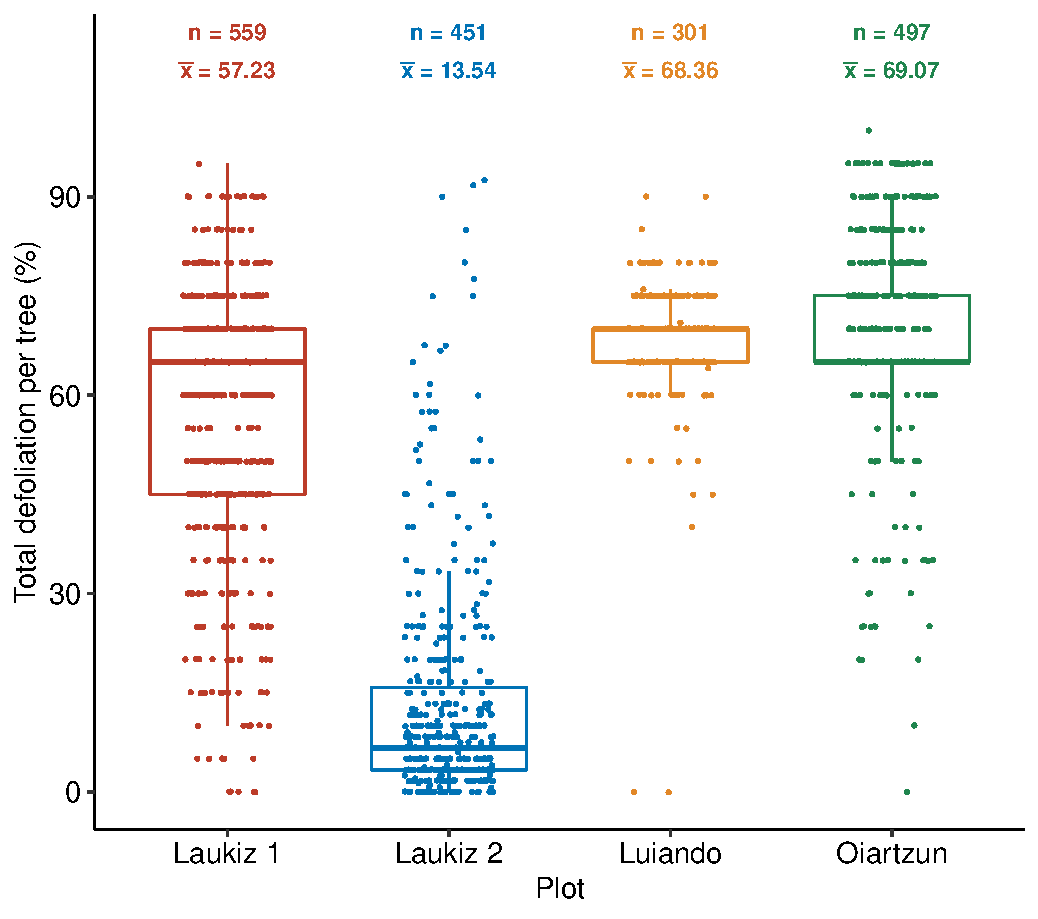
\includegraphics[width=0.7\textwidth] {defoliation-distribution-plot-1.pdf}
		\caption{Response variable ``defoliation of trees'' for plots~Laukiz1, Laukiz2, Luiando and Oiartzun. \texttt{n} is the total number of trees in each plot, and $\bar{x}$ the mean defoliation. Values for Laukiz1, Luiando and Oiartzun were observed in 5\% intervals; for Laukiz2 defoliation was observed at multiple heights and then averaged, leading to smaller defoliation differences than 5\%.}\label{fig:defol-distr}
	\end{center}
\end{figure}

\subsubsection{In-situ data}

The \textit{Pinus radiata} plots of this study, namely Laukiz1, Laukiz2, Luiando and Oiartzun, are located in the northern part of the Basque Country (\autoref{fig:study_area}).
Oiartzun has the largest number of observations ($n = 559$ trees) while Laukiz2 is the largest in area (1.44~ha).
All plots besides Luiando are located within 100~km from the coast (\autoref{fig:study_area}).
A total of 1808 observations are available (Laukiz1: 559, Laukiz2: 451, Luiando: 301, Oiartzun: 497).
Field surveys were conducted in September 2016 by experienced forest pathologists.
Defoliation was measured in 5\% steps through visual inspection with the help of a score card.
For Laukiz2, values at three height levels (bottom, mid, top) were available and averaged into an overall defoliation value, resulting in values that are not multiples of 5\% (e.g., 8.33\%).
The magnitude of human observer errors in such surveys, including the present one, is not precisely known and has being discussed for many years \cite{innes1993}.
\cite{maclean1982} estimated human observer errors in defoliation surveys to range between 7\% and 18\%.

\begin{figure*} [ht!]
	\begin{center}
		\centering
		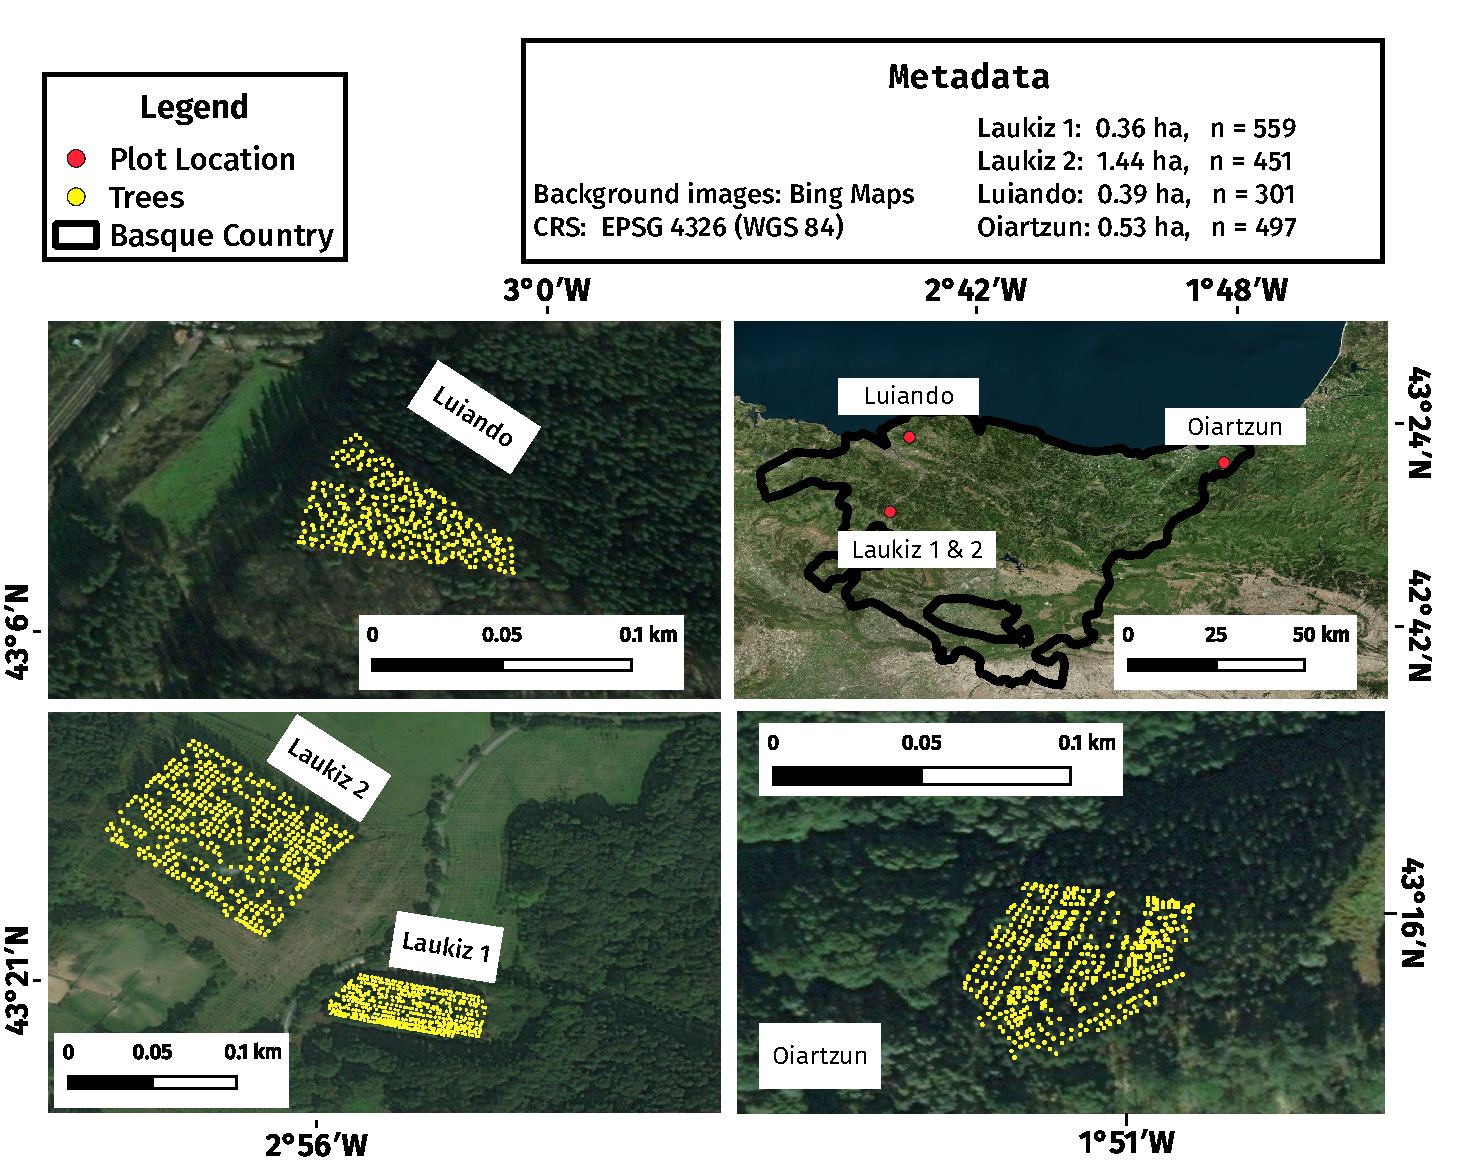
\includegraphics[width=\textwidth] {study-area-hyperspectral.pdf}
		\caption{Study area maps showing information about location, size and spatial distribution of trees for all plots (Laukiz1, Laukiz2, Luiando, Oiartzun). The background maps give a visual impression of the individual plot area but do not necessarily represent the plot's state during data acquisition.}\label{fig:study_area}
	\end{center}
\end{figure*}

%\begin{figure} [t!]
%	\begin{center}
%		\includegraphics[width=0.7\textwidth] {defol-grid-3000px.jpg}
%		\caption{Example trees showing different levels of defoliation as interpreted by the surveyor: 10 \% (top-left), 20 \% (top-right), 40 \% (bottom-left), 60-70 \% (bottom-right).}
%		\label{fig:defol-trees}
%	\end{center}
%\end{figure}

\subsubsection{Hyperspectral data}

The airborne hyperspectral data was acquired by an AISA EAGLE-II sensor during two flight campaigns on September 28th and October 5, 2016 at noon.
All preprocessing steps (geometric, radiometric, atmospheric) were conducted by the \ac{ICGC}.
The first four bands were corrupted, leaving 122 bands with valid information.
Additional metadata information is available in \autoref{tab:hyperparameter_metadata}.

% parameter limits

\begin{table}[t]
	\centering
	\caption[t]{Specifications of hyperspectral data.}
	\begingroup
	\begin{tabular}{ll}
		\\
		Characteristic         & Value                               \\
		\toprule
		Geometric resolution   & 1~m                                 \\
		Radiometric resolution & 12 bit                              \\
		Spectral resolution    & 126 bands (404.08~nm~--- 996.31~nm) \\
		Correction:            & Radiometric, geometric, atmospheric
	\end{tabular}
	\endgroup\label{tab:hyperparameter_metadata}
\end{table}

\subsection{Derivation of indices}

To use the full potential of the hyperspectral data, all possible vegetation indices supported by the R package \texttt{hsdar} (89 in total) as well as all possible \ac{NRI} combinations were calculated.
NRIs follow the \ac{OMNBR} concept of data-driven information extraction from narrow-band indices of hyperspectral data \cite{thenkabail2000,thenkabail2018}.
While various index formulations such as band ratios or normalized ratios are available, indices involving the same bands are strongly correlated.
Since the widely\ used NDVI index belongs to the group of normalized ratio indices (NRIs), which are implemented in the \texttt{hsdar} R package, we used the following normalized difference index (NDI) formula to combine all pairs of reflectances:

\begin{equation}
	NRI_{i,j} = \frac{band_{i} - band_{j}}{band_{i} + band_{j}}
\end{equation}

\noindent
where \(i\) and \(j\) are the respective band numbers.

\bigbreak{}

To account for geometric offsets within the hyperspectral data, which were reported by \ac{ICGC} to be potentially up to one meter, a buffer of one meter radius around the centroid of each tree was used when extracting the reflectance values.
A pixel was considered to fall into a tree's buffer zone if the centroid of the respective pixel was touched by the buffer.
The pixel values within a buffer zone were averaged and formed the final reflectance value of a single tree and were used as the base information to derive all additional feature sets.
In total, \(\frac{121*122}{2} = 7381\) NRIs were calculated.

\subsection{Feature selection}

High-dimensional, feature-rich datasets come with several challenges for both model fitting and evaluation.

\begin{itemize}
	\item Model fitting times increase.
	\item Noise is possibly introduced into models by highly correlated variables \cite{johnstoneiainm.2009}.
	\item Model interpretation and prediction become more challenging \cite{johnstoneiainm.2009}.
\end{itemize}

To reduce the feature space of a dataset, several conceptually differing approaches exist: wrapper methods, filters, penalization methods (lasso and ridge), and \ac{PCA} \cite{bommert2020, das2001, guyon2003, jolliffe2016}.
In contrast to wrapper methods, filters have a much lower computational cost, and their tuning can be added to the hyperparameter optimization step.
In addition, filters are less known than wrapper methods and in recent years, ensemble filters were introduced which have shown promising results compared to single filter algorithms \cite{drotar2017}.
These two points mainly led to the decision to focus on filter methods for this work and evaluate their effectiveness on highly\ correlated, high-dimensional datasets.
Due to this focus, only this subgroup of feature selection methods will be introduced in greater detail in the following sections.

\subsubsection{Filter methods}

% Filter methods
The concept of filters originates from the idea of ranking features following a score calculated by an algorithm \cite{guyon2003}.
Some filter methods can only deal with specific types of variables (e.g., numeric or nominal).
Filters only rank features, they do not decide which covariates to drop or keep \cite{drotar2015}.
The decision which features to keep for model fitting can be integrated into the optimization phase during model fitting, along with hyperparameter tuning.
Thus, the number of top-ranked features to be included in the model is treated as an additional hyperparameter of the model.
This hyperparameter is tuned to optimize the model's performance.

% Ensemble filter methods
Beyond the use of individual filter methods to rank and select features, recent studies have shown that combining several filters by using statistical operations such as 'minimum' or 'mean' may enhance the predictive performance of the resulting models, especially when applied to multiple datasets \cite{abeel2010, drotar2017}.
This approach is referred to as 'ensemble filtering' \cite{dietterich2000}.
Ensemble filters align with the recent rise of the ensemble approach in ML, which uses the idea of stacking to combine the predictions of multiple models, aiming to enhance predictive performance \cite{polikar2012, feurer2015, bolon-canedo2019}.
In this work the Borda ensemble filter was used \cite{drotar2017}.
Its overall feature order is determined by the sum of filter ranks of all individual filters in the ensemble.

% Ensuring a fair weighting in the ensemble
Filter methods can be categorized based on three binary criteria: multivariate or univariate feature use, correlation or entropy-based importance weighting, and linear and non-linear filter methodology.
Care needs to be taken to not weigh certain classes more than others in the ensemble as otherwise the ranking will be biased.
In this study this was taken care of by checking the rank correlations (Spearman's correlation) of the generated feature rankings of all methods against each other.
If filter pairs showed a correlation of 0.9 or higher, only one of the two was included in the ensemble filter, selecting it at random.

\subsubsection{Description of used filter methods}

Filter methods can be classified as follows (\autoref{tab:filter-methods}):

\begin{itemize}
	\item Univariate/multivariate (scoring based on a single variable/multiple variables).
	\item Linear/non-linear (usage of linear/non-linear calculations).
	\item Entropy/correlation (scoring based on derivations of entropy or correlation-based approaches).
\end{itemize}

% filter methods
\begin{table}[b!]
	\centering
	\caption{List of filter methods used in this work, their categorization and scientific reference.}
	\label{tab:filter-methods}
	\begingroup\footnotesize
	\begin{adjustbox}{width={0.7\textwidth},totalheight={\textheight},keepaspectratio}
		\begin{tabular}{lll}
			\\
			Name                                         & Group                             & Ref.               \\
			\toprule
			Linear correlation (Pearson)                 & univariate, linear, correlation   & \cite{pearson1901} \\
			Information gain                             & univariate, non-linear, entropy   & \cite{quinlan1986} \\
			Minimum redundancy, maximum relevance        & multivariate, non-linear, entropy & \cite{zhao2013}    \\
			Carscore                                     & multivariate, linear, correlation & \cite{zuber2011}   \\
			Relief                                       & multivariate, linear, entropy     & \cite{kira1992}    \\
			Conditional minimal information maximization & multivariate, linear, entropy     & \cite{fleuret2004}
		\end{tabular}
	\end{adjustbox}
	\endgroup
\end{table}

The filter 'Information Gain' in its original form is only defined for nominal response variables:

\begin{equation}
	H(Class) + H(Attribute) - H(Class, Attribute)
\end{equation}

where \(H\) is the conditional entropy of the response variable (class or Y) and the feature (attribute or X), respectively.
$H(X)$ is Shannon's Entropy \cite{shannon1948} for a variable X and $H(X, Y)$ is a joint Shannon's Entropy for a variable X with a condition to Y.
$H(X)$ itself is defined as

\begin{equation}
	H(X) = - \sum_{i=1}^{n} P(x_i)\log_bP(x_i)
\end{equation}

where $b$ is the base of the logarithm used, most commonly 2.

In order to use this method with a numeric response (percentage defoliation of trees), the variable was discretized into equal bins \texttt{\(n_{bin}\) = 10} and treated as a categorical variable.

\subsection{Benchmarking design}

\subsubsection{Algorithms}

The following learners were used in this work:

\begin{itemize}
	\item  Extreme Gradient Boosting (XGBoost)
	\item  Random Forest (RF)
	\item  Penalized Regression (with L1/lasso and L2/ridge penalties)
	\item  Support Vector Machine (SVM, radial basis function Kernel)
	\item  Featureless learner
\end{itemize}

RF and SVM are well-established algorithms and widely used in environmental remote sensing.
Extreme Gradient Boosting (commonly abbreviated as XGBoost) has shown promising results in benchmarking studies in recent years.
Penalized regression is a statistical modeling technique capable of dealing with highly\ correlated covariates by penalizing the model coefficients \cite{hastie2001}.
Common penalties are 'lasso' (L1) and 'ridge' (L2).
Ridge regression does not remove variables from the model (penalization to zero), but it shrinks them towards zero, keeping them in the model.
A featureless learner was included for a baseline comparison.

In total, the benchmarking grid consisted of 156 experiments (6 feature sets $\times$ 3~ML algorithms $\times$ 8 feature-selection methods and for the L1/L2 models, 6 feature sets $\times$ 2 models.
The selected hyperparameter settings are shown in appendix \autoref{tab:hyperparameter_limits}.
All code and data are included in the research compendium of this study (\url{https://doi.org/10.5281/zenodo.2635403}).

\subsubsection{Feature sets}

Three feature sets were used in this study, each representing a different approach to feature engineering:

\begin{itemize}
	\item The raw hyperspectral band information (HR): no feature engineering %chktex 13
	\item Vegetation Indices (\ac{VI}s): expert-based feature engineering
	\item Normalized Ratio Indices (\ac{NRI}s): data-driven feature engineering
\end{itemize}

The idea of splitting the features into different sets originated from the question whether feature-engineered indices derived from reflectance values have a positive effect on model performance.
Peña et al. 2017 \cite{pena2017} is an exemplary study which used this approach in a spectro-temporal setting.
Benchmarking learners on these feature sets while keeping all other variables such as model type, tuning strategy and partitioning method fixed makes it possible to draw conclusions on their individual impact.
Each feature set has distinct capabilities that differentiate it from the others.
This can have both a positive and negative effect on the resulting performance, which is one question this study aims to explore.
For example, feature set VI misses certain parts of the spectral range as the chosen indices only use specific spectral bands.
Feature set NRI will introduce highly\ correlated features, for which some algorithms may be more suitable than others.

In addition to these individual feature sets, the following combinations of feature sets were also compared:

\begin{itemize}
	\item HR + VI %chktex 13
	\item HR + NRI
	\item HR + VI + NRI
\end{itemize}

Some individual features were removed before using the datasets for modeling when being numerically equivalent to another feature based on the pairwise correlation being greater than $1 - 10^{-10}$.
This preprocessing step reduced the number of covariates for feature set~VI to 86 (from 89).
This decision was made to prevent numerical issues that may occur in the subsequent tuning, filtering and model fitting steps when offering features with a pairwise correlation of (almost) one.
The remaining features were then used as input for the filter-based feature selection within the CV.


\subsubsection{Hyperparameter optimization}

Hyperparameters were tuned using \ac{MBO} within a nested spatial \ac{CV} \cite{mlrmbo, binder2020, schratz2019}.
In MBO, first \textit{n} hyperparameter settings are randomly chosen from a user-defined search space.
After these \textit{n} settings have been evaluated, one new setting, which is going to be evaluated next, is proposed by a fitted surrogate model (by default, a kriging method).
This strategy continues until a user-defined stopping criterion is satisfied \cite{hutter2011, jones1998}.

In this work, an initial design of 30 randomly drawn hyperparameter settings in combination with a stopping criterion of 70 iterations was used, resulting in a total budget of 100 evaluated hyperparameter settings per fold.
The advantage of this tuning approach is a substantial reduction of the tuning budget that is required to find a setting close to the global optimization minimum.
\ac{MBO} may outperform methods that do not use information from previous iterations, such as random search or grid search \cite{bergstra2012}.
Tuning ranges used in this work are shown in \autoref{tab:hyperparameter_limits}.

To optimize the number of features used for model fitting, the percentage of features was added as a hyperparameter during the optimization stage \cite{binder2020}.
For \ac{PCA}, the number of principal components was tuned.
%The RF hyperparameter \texttt{\(m_{try}\)} was re-expressed as $m_{try} = p^x_{try}$.
The RF hyperparameter \texttt{\(m_{try}\)} was re-expressed as $m_\textrm{try} = p_\textrm{sel}^t$, a function of the number of selected features, $p_\textrm{sel}$.
It was thus tuned on a logarithmic scale by varying $t$ between 0 (i.e., $m_\textrm{try} = 1$) and 0.5 (i.e., $m_\textrm{try}=\sqrt{p_\textrm{sel}}$).
This was necessary to ensure that \texttt{\(m_{try}\)} did not exceed the number of features available after optimizing the feature percentage during tuning.

\subsubsection{Spatial resampling}

A spatial nested cross-validation on the plot level was chosen to account for spatial autocorrelation within the plots and assess model transferability to different plots \cite{schratz2019, sperrorest}.
The \ac{RMSE} was chosen as the error measure.
Each plot served as one cross-validation fold, resulting in four iterations in total.
The inner level of cross-validation for hyperparameter tuning also used plot-level cross-validation.

\subsection{Feature importance and feature effects}

Estimating feature importance for datasets with highly correlated features is a challenging task for which numerous model-specific and model-agnostic approaches exist \cite{friedman2001, hastie2001, greenwell2018}.
The strong correlations among features make it challenging to calculate an unbiased estimate for single features \cite{molnar2019}.
Methods like \ac{PDP} or permutation-based approaches may produce unreliable estimates in such scenarios because unrealistic combinations of feature values are created \cite{molnar2019}.
The development of robust methods that enable an unbiased estimation of feature importance for highly correlated variables are subject to current research \cite{brenning2021}.

In this work, permutation-based feature importance was calculated to estimate feature importance or effects \cite{apley2019}.
With the limitations in mind when applied to correlated features, the aim was to get a general overview of the feature importance of the hyperspectral bands while trying to avoid an over-interpretation of results.
The best-performing algorithm on the HR task (i.e., SVM) was used for the feature importance calculation.

%\subsection{Linking feature importance to wavelength regions}

To facilitate interpretation, the ten most important indices of the best performing models using feature sets HR and VI were linked to the spectral regions of the hyperspectral data that went into their calculation.
The aim was to visualize the most important features along the spectral curve of the plots to better understand which spectral regions were most important for the model.

\subsection{Research compendium}

All tasks of this study were conducted using the open-source statistical programming language R \cite{rcoreteam2019}.
A complete list of all R packages used in this study can be found in the linked repositories mentioned in the next paragraph.
Due to space limitations, only selected packages with high impact on this work will be explicitly cited.

The algorithm implementations of the following packages have been used: xgboost \cite{chen2016} (\textit{Extreme Gradient Boosting}), kernlab \cite{kernlab} (Support Vector Machine) and glmnet \cite{glmnet} (penalized regression).
The filter implementations of the following packages have been used: praznik \cite{praznik}, FSelectorRcpp \cite{fselectorrcpp}.
Package mlr \cite{mlr} was used for all modeling related steps.
drake \cite{drake} was used for structuring the work and for reproducibility.
This study is available as a research compendium on Zenodo (\url{10.5281/zenodo.2635403}).
Apart from the availability of code and manuscript sources, a static webpage is available at (\url{https://pat-s.github.io/2019-feature-selection}), which includes additional side analyses that were carried out during the creation of this study.

%%%%%%%%%%%%%%%%%%%%%%%%%%%%%%%%%%%%%%%%%%
\section{Results}

\subsection{Principal component analysis of feature sets}

PCA was used to assess the complexity of the three feature sets.
Depending on the feature set, 95\% of the variance is explained by two (HR), twelve (VI) and 42 (NRI) \ac{PC}s.
HR features are therefore highly redundant, while the applied feature transformations enrich the data set, at least from an exploratory linear perspective.

\subsection{Predictive performance}

% - RMSE around 27
% - MBO tuned penalized methods are substantially worse
Overall, the response variable \enquote{tree defoliation} could be modeled with an \ac{RMSE} of 28 percentage points (p.p.) (\autoref{fig:perf-result}).
SVM showed almost no differences in RMSE across feature sets whereas other learners (RF, SVM, XGBoost, lasso and ridge) differed up to five p.p. (\autoref{fig:perf-result}).
SVM showed the best overall performance with a mean difference of around three p.p. to the next best model (XGBoost) (\autoref{tab:best-learner-perf}).
Performance differences between test folds were large: Predicting on Luiando resulted in an RMSE of 9.0 p.p. for learner SVM (without filter) but up to 54.3 p.p. when testing on Laukiz2 (\autoref{tab:svm-single-fold-perf}).

% feature sets
% - no substantial difference between feature sets
% - combining feature sets has only small impact
% - expert based feature sets show no better result than data-driven ones
% - penalized methods seem to have problems with VI feature set
The combination of feature sets showed small increases in performance for some learners.
XGBoost scored slightly better on the combined datasets HR-NRI, NRI-VI and HR-NRI-VI, respectively, compared to their standalone variants (NRI, VI) (\autoref{fig:perf-result}).
However, the best performances for RF and XGBoost were scored on NRI and HR, respectively.
RF showed a substantial performance increase when using only NRI compared to all other feature sets whereas for XGBoost the worst performances were associated with the VI and NRI only feature sets (\autoref{fig:perf-result}).

% learner
% - SVM Info Gain is the overall winner
% - Combined sets do not help for XBoost and Ridge
% - RF NRI quite strong
SVM combined with the \enquote{Information Gain} filter achieved the best overall performance (RMSE of 27.915 p.p.) (\autoref{tab:perf-top-10}).
%L1 penalized regression showed slightly better results in three out of six tasks when being optimized using the package internal 10-fold CV compared to MBO (RMSE of 50 vs 58).
Regression with ridge (L2) and lasso (L1) penalties showed their best performances on the NRI feature set (\autoref{tab:best-learner-perf}).
Combining feature sets for lasso and ridge did not help to increase performance, and while there was no substantial difference for lasso, the performance of ridge improved by around two percentage points.
XGBoost showed very poor performances for some feature sets and fills the last\ ten places of the ranking (\autoref{tab:perf-worst-10}).
Especially when combined with PCA, the algorithm was not able to achieve adequate performances.

% filters
% - influence varies based on algorithm and task (SVM no influence, RF medium, XGB medium)
% - no substantial decrease in performance when using filters
% - no advantage of ensemble borda filter compared to others
Effects of filter methods on performance differed greatly between algorithms:
SVM showed no variation in performance across filters (\autoref{fig:filter-effects-no-filter}).
The use of filters for RF resulted in a substantial increase in performance in all tasks, especially on the HR feature set where all filters showed an improved score compared to using no filter (\autoref{fig:filter-effects-no-filter}).
XGBoost's performance depended strongly on feature selection: In two out of six tasks (HR, VI), using no filter resulted in the worst performance.
XGBoost showed the highest overall differences between filters for a single task: for feature set HR, the range is up to 13 p.p. (\enquote{CMIM} vs. \enquote{no filter}) (\autoref{fig:filter-effects-no-filter}).

% filter vs. no filter
% - Substantial effect for XGBoost and RF
% - SVM unaffected
When comparing the usage of filters against using no filter at all, there were no instances in which a non-filtered model scored a better performance than the best filtered one (\autoref{fig:filter-effects-no-filter}).
For SVM, all filters and \enquote{no filter} achieved roughly the same performance on all tasks.

% Borda vs. other filters
% - most often among the first best filters for each task
% - never the best
The Borda ensemble filter was not able to score the best performance in any learner/filter setting (\autoref{fig:filter-effects-borda}).
For RF and XGBoost, it most often ranked within the better half among all filters of a specific task.

% Selected percentage of features across plots
The number of features selected during model optimization strongly varied across learners and plots.
RF selected the least features of all three learners, and with the exception of Oiartzun, only one or two variables were selected.
SVM used 210 features or more in all instances and selected between 16\% (Laukiz1) and 81\% (Oiartzun) of the features (\autoref{tab:tune-perc-sel-features}).
XGBoost also favored using several hundred features with the exception of Laukiz2 for which only 14 (0.96\%) were selected.

% latex table top 10 absolute performances
% latex table generated in R 4.0.4 by xtable 1.8-4 package
\begin{table}[ht!]
\centering
\caption{Best ten results among all combinations, sorted in ascending order of RMSE} 
\label{tab:perf-top-10}
\begin{tabular}{rlllrrr}
  \hline
 & Task & Model & Filter & RMSE & SE (RMSE) & $R^2$ \\ 
  \hline
1 & HR-NRI-VI & SVM & Relief & 28.09 & 18.95 & -3.04 \\ 
  2 & HR & SVM & Borda & 28.12 & 19.12 & -3.04 \\ 
  3 & HR & SVM & Car & 28.12 & 19.12 & -0.15 \\ 
  4 & HR & SVM & CMIM & 28.12 & 19.12 & -0.15 \\ 
  5 & HR & SVM & Info Gain & 28.12 & 19.12 & -0.15 \\ 
  6 & HR & SVM & MRMR & 28.12 & 19.12 & -0.17 \\ 
  7 & HR & SVM & Relief & 28.12 & 19.12 & -0.17 \\ 
  8 & HR-NRI-VI & SVM & CMIM & 28.12 & 19.18 & -9.33 \\ 
  9 & HR-NRI-VI & SVM & Car & 28.12 & 19.12 & -9.30 \\ 
  10 & NRI-VI & SVM & CMIM & 28.12 & 19.12 & -0.15 \\ 
   \hline
\end{tabular}
\end{table}


% latex table worst 10 absolute performances
% latex table generated in R 4.0.4 by xtable 1.8-4 package
\begin{table}[ht!]
\centering
\caption{Worst ten results among all combinations, sorted in decreasing order of RMSE} 
\label{tab:perf-worst-10}
\begin{tabular}{rlllrrr}
  \hline
 & Task & Model & Filter & RMSE & SE (RMSE) & $R^2$ \\ 
  \hline
1 & NRI-VI & XGBoost & PCA & 47.19 & 9.17 & -39.30 \\ 
  2 & HR-NRI-VI & XGBoost & PCA & 46.30 & 5.79 & -5.30 \\ 
  3 & NRI & XGBoost & PCA & 45.96 & 8.28 & -12.79 \\ 
  4 & VI & XGBoost & PCA & 45.73 & 7.54 & -37.70 \\ 
  5 & VI & XGBoost & No Filter & 45.08 & 6.95 & -5.24 \\ 
  6 & HR & XGBoost & No Filter & 45.08 & 5.26 & -22.39 \\ 
  7 & HR-NRI-VI & XGBoost & Relief & 44.76 & 5.54 & -4.80 \\ 
  8 & HR-NRI & XGBoost & PCA & 43.14 & 7.21 & -9.12 \\ 
  9 & HR-NRI & XGBoost & MRMR & 42.84 & 6.73 & -4.95 \\ 
  10 & HR-NRI & XGBoost & Pearson & 42.44 & 6.45 & -20.70 \\ 
   \hline
\end{tabular}
\end{table}


% latex table best performance per learner
% latex table generated in R 4.0.4 by xtable 1.8-4 package
\begin{table}[ht!]
\centering
\caption{The overall best individual learner performance across any task and filter method for RF, SVM, XGBoost, Lasso and Ridge, sorted ascending by RMSE (p.p.) including the respective standard error (SE) of the cross-validation run. For 	exttt{regr.featureless} the Task is no applicable and was therefore removed.} 
\label{tab:best-learner-perf}
\scalebox{0.9}{
\begin{tabular}{rlllrr}
  \hline
 & Task & Model & Filter & RMSE & SE \\ 
  \hline
1 & HR & SVM & Relief & 28.119 & 19.123 \\ 
  2 & NRI & Lasso-MBO & No Filter & 31.165 & 15.025 \\ 
  3 & NRI & Ridge-MBO & No Filter & 31.165 & 15.025 \\ 
  4 & - & regr.featureless & No Filter & 31.165 & 15.025 \\ 
  5 & HR & RF & Relief & 31.246 & 14.956 \\ 
  6 & HR & XGBoost & Car & 34.071 & 13.571 \\ 
   \hline
\end{tabular}
}
\end{table}


% latex table top 20 absolute performances
% latex table generated in R 4.0.4 by xtable 1.8-4 package
\begin{table}[ht!]
\centering
\caption{Test fold performances for learner SVM on the HR dataset without using a filter. For each row, the model was trained on observations from all others plots but the given one and tested on the observations of the given plot.} 
\label{tab:svm-single-fold-perf}
\begin{tabular}{rrrl}
  \hline
 & Plot & RMSE & Test Plot \\ 
  \hline
1 &   1 & 28.12 & Laukiz1 \\ 
  2 &   2 & 54.26 & Laukiz2 \\ 
  3 &   3 & 9.00 & Luiando \\ 
  4 &   4 & 21.17 & Oiartzun \\ 
   \hline
\end{tabular}
\end{table}


% latex table percentage of selected features during tuning
% latex table generated in R 4.0.4 by xtable 1.8-4 package
\begin{table}[ht!]
\centering
\caption{Selected feature portions during tuning for the best performing learner-filter settings (SVM Relief, RF Relief, XGBoost CMIM) across folds for task HR-NRI-VI, sorted by plot name. 	exttt{#} denotes the absolute number of features selected and 'Features (	exttt{%})' refers to the percentage relative to the overall features available (7675). Results were estimated in a separate model tuning step, not within the main cross-validation comparison.} 
\label{tab:tune-perc-sel-features}
\begin{tabular}{llrrr}
  \toprule
Learner & Test Plot & Features (\%) & \# & RMSE \\ 
  \midrule
\multirow{4}{*}{\specialcell{RF \\ Relief}} & Luiando & 99.97268 & 301 & 41.73 \\ 
   & Laukiz2 & 93.37086 & 422 & 17.12 \\ 
   & Laukiz1 & 0.21573 & 2 & 33.21 \\ 
   & Oiartzun & 0.00405 & 1 & 37.20 \\ 
  \midrule\multirow{4}{*}{\specialcell{XGB \\ CMIM}} & Luiando & 30.84900 & 93 & 33.36 \\ 
   & Laukiz1 & 98.12213 & 549 & 45.59 \\ 
   & Oiartzun & 83.61298 & 416 & 41.01 \\ 
   & Laukiz2 & 0.51526 & 3 & 15.24 \\ 
  \midrule\multirow{4}{*}{\specialcell{SVM \\ Relief}} & Laukiz1 & 0.06200 & 1 & 35.49 \\ 
   & Oiartzun & 4.10636 & 21 & 31.03 \\ 
   & Luiando & 20.73514 & 63 & 37.19 \\ 
   & Laukiz2 & 23.92820 & 108 & 14.89 \\ 
   \bottomrule
\end{tabular}
\end{table}


% plot performance results
\begin{figure} [t!]
	\centering
	\begin{center}
		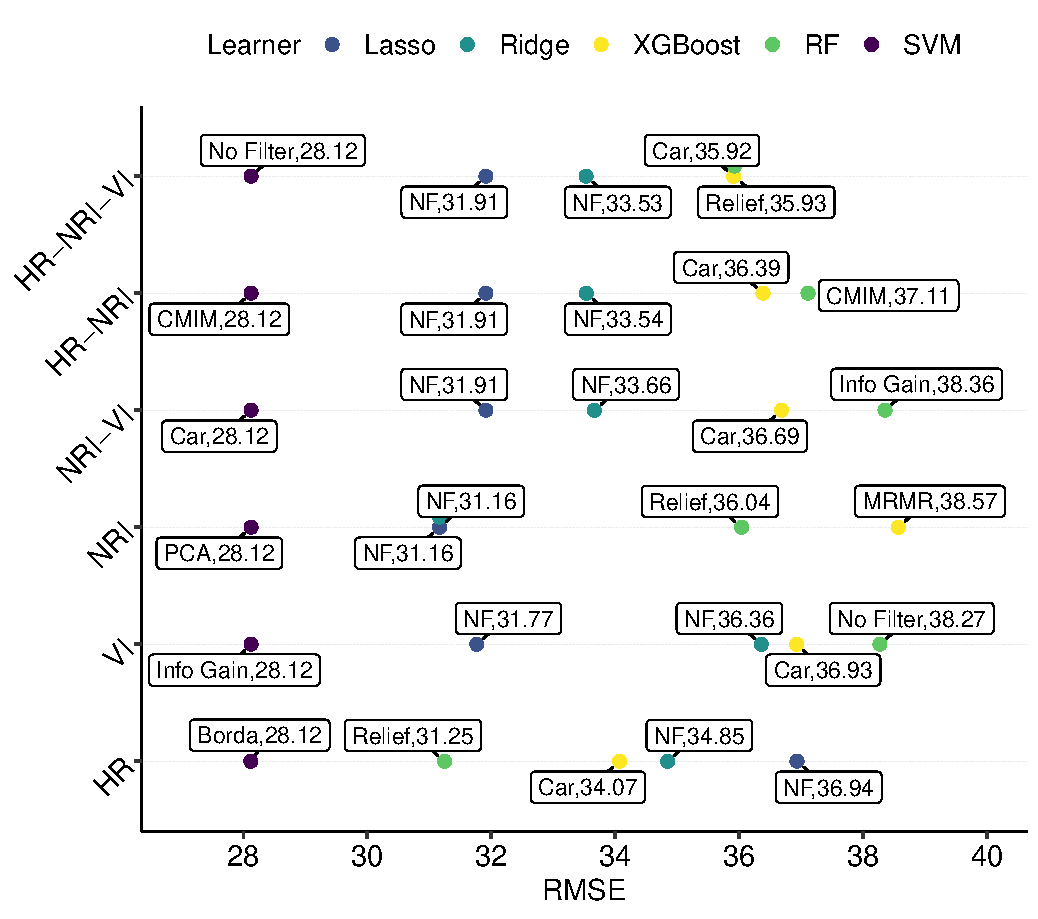
\includegraphics[width=0.7\textwidth] {performance-results-1.pdf}
		\caption{Predictive performance in RMSE (p.p.) of models across tasks. Different feature sets are shown on the y-axis. Labels show the feature selection method (e.g., NF = no filter, Car = 'Carscore', Info Gain = 'Information Gain', Borda = 'Borda').}\label{fig:perf-result}
	\end{center}
\end{figure}

% plot no filter vs all other filters for each model and task
\begin{figure} [t!]
	\centering
	\begin{center}
		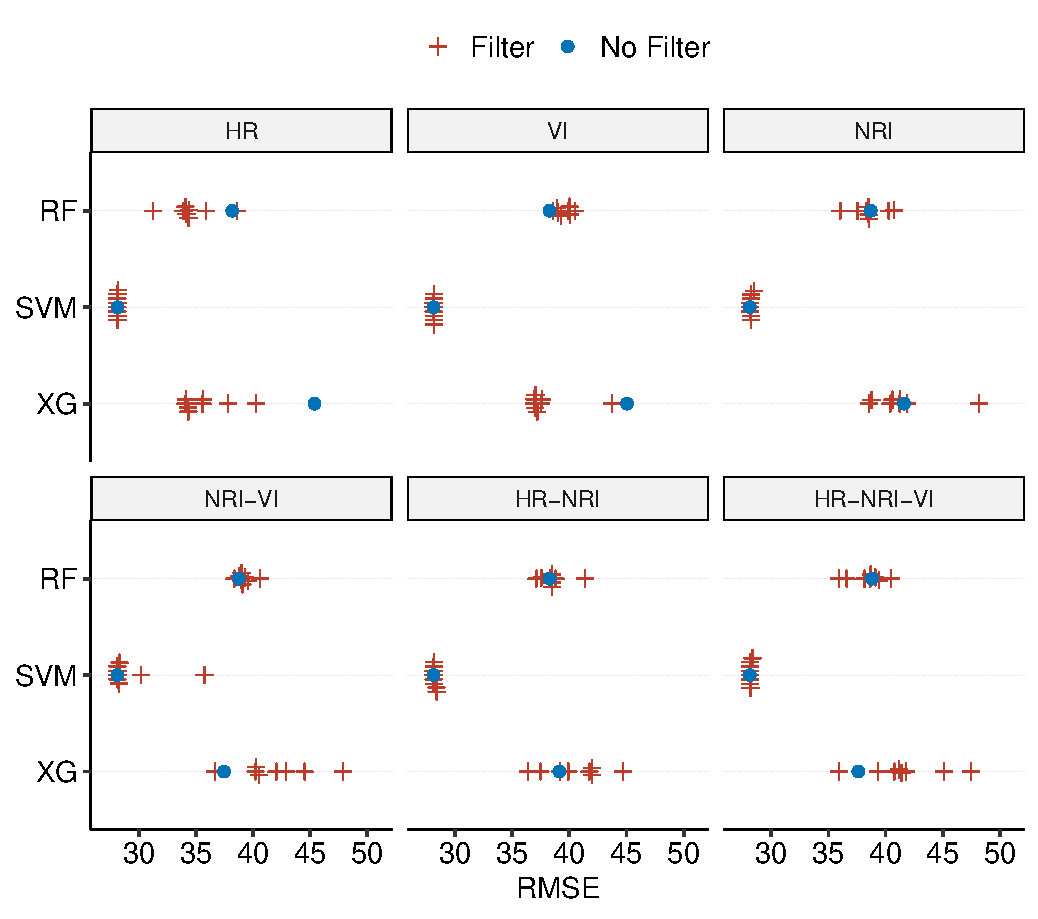
\includegraphics[width=0.7\textwidth] {filter-effect-all-vs-no-filter-1.pdf}
		\caption{Model performances in RMSE across all tasks, split up in facets, when using no filter method (blue dot) compared to any other filter method (red cross) for learners RF, SVM and XGBoost (XG)}\label{fig:filter-effects-no-filter}
	\end{center}
\end{figure}

% plot Borda vs all other filters for each model and task
\begin{figure} [t!]
	\centering
	\begin{center}
		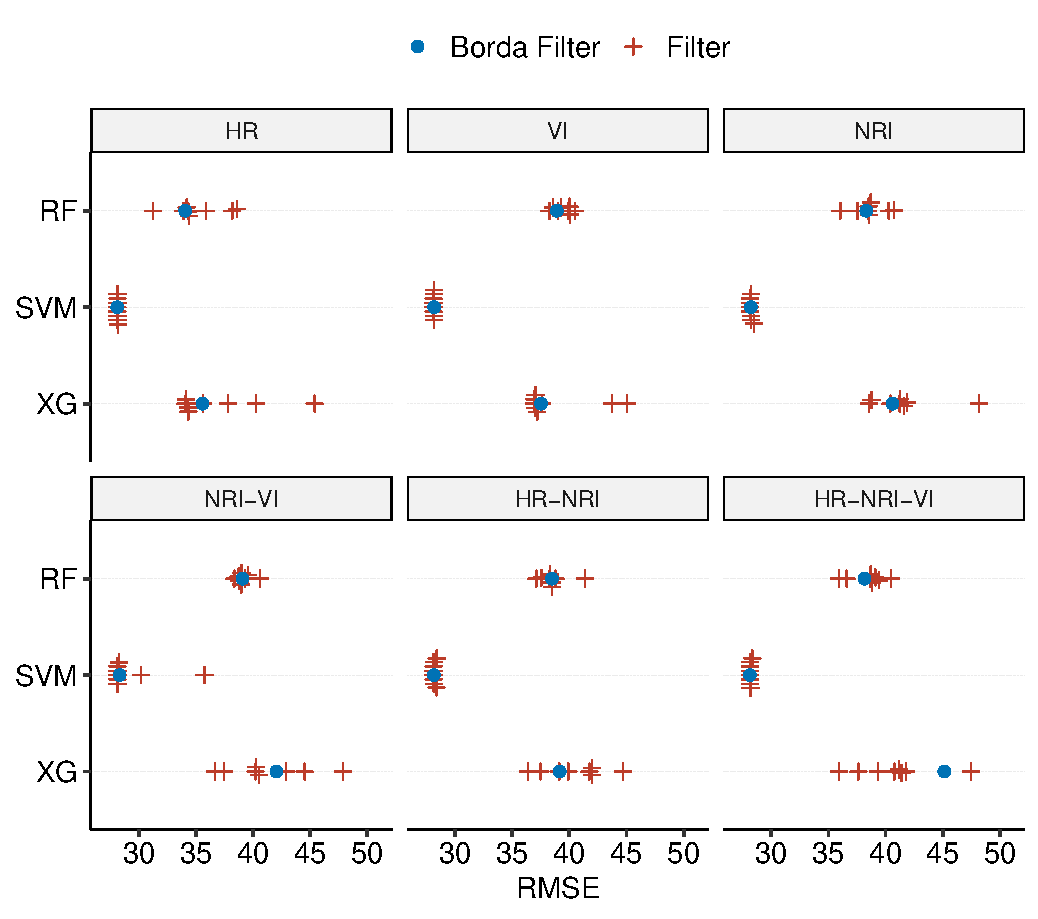
\includegraphics[width=0.7\textwidth] {filter-effect-all-vs-borda-filter-1.pdf}
		\caption{Predictive performances in RMSE (p.p.) when using the Borda filter method (blue dot) compared to any other filter (red cross) for each learner across all tasks.}\label{fig:filter-effects-borda}
	\end{center}
\end{figure}

\subsection{Variable importance}

\subsubsection{Permutation-based Variable Importance}

% Variable Importance
% - VI: Vogelmann indices are best
% - All: Clustering around the red edge (700 - 750 nm)
% - Overall highest: 1.7 RMSE decrease - not that much

The most important features for datasets HR and VI showed an average decrease in RMSE of 1.06 p.p. (HR, B65) and 1.93 p.p. (VI, Vogelmann2) when permuted (\autoref{fig:fi-permut-vi-hr}).
For the HR dataset, most (i.e., six out of ten) relevant features clustered around the infrared region (920~nm - 1000~nm), while for VI, eight out of ten concentrate within the wavelength range of 700~nm - 750~nm (the so\-/called \enquote{red edge}).
For HR, four features in the infrared region (920~nm - 1000~nm) were identified by the model to be most important, being associated with a mean decrease in RMSE of around 1 p.p.
Overall, apart from the top five features, the vast majority of features showed only a small importance with average decreases in RMSE below 0.5 p.p.

% permutation based var imp for datasets HR and VI
\begin{figure*} [ht!]
	\centering
	\begin{center}
		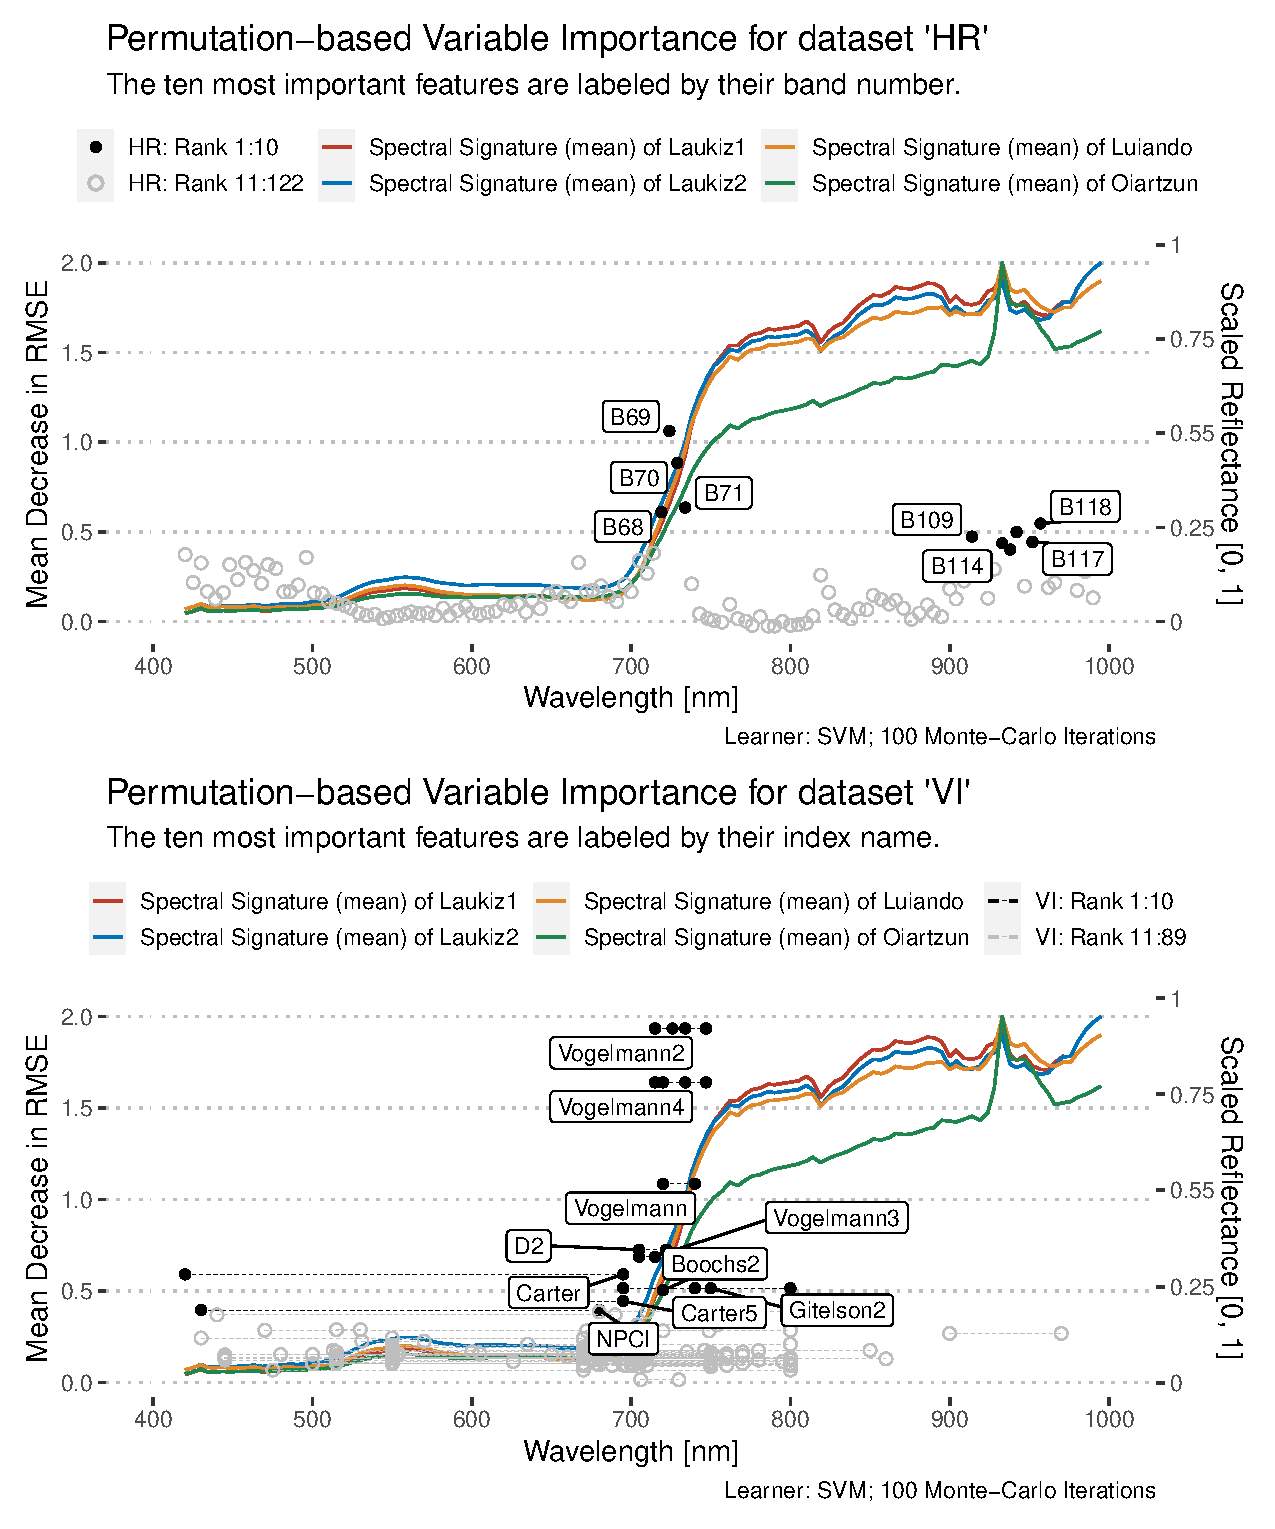
\includegraphics[width=0.9\textwidth] {fi-permut-vi-hr-1.pdf}
		\caption{Variable importance for feature sets HR and VI: Mean decrease in RMSE for one\ hundred feature permutations using the SVM learner. The wavelength range on the x-axis matches the range of the hyperspectral sensor (400~nm - 1000~nm). For each dataset, the ten most important features were highlighted as black dots and labeled by name. Gray dots represent features from importance rank~11 to last. The spectral signature (mean) of each plot was added as a reference on a normalized reflectance scale [0, 1] (secondary y-axis). VI features were decomposed into their individual formula parts; all instances being connected via dashed lines. Each VI feature is composed out of at least two instances.}\label{fig:fi-permut-vi-hr}
	\end{center}
\end{figure*}


%%%%%%%%%%%%%%%%%%%%%%%%%%%%%%%%%%%%%%%%%%
\section{Discussion}

\subsection{Predictive Performance}

The best overall performance achieved in this study (SVM with the \enquote{Info Gain} filter, RMSE~27.915 p.p.) has to be seen in the light of model overfitting (see \autoref{subsec:perf-plot-char}).
Leaving out the performance on Laukiz2 when aggregating results, the mean RMSE would be around 19 p.p.
However, leaving out a single plot would also change the prediction results for the other plots because the observations from Laukiz2 would not be available for model training.
Due to the apparent presence of model overfitting in this study, it is suggested that more training data representing a greater variety of situations is needed.
A model can only make robust predictions if it has learned relationships across the whole range of the response.
Hence, care should be taken when predicting on the landscape scale using models fitted on this dataset due to their lack of generalizability caused by the limitations of the available training data.
However, when inspecting the fold\-/level performances, it can be concluded that the models performed reasonably well predicting defoliation greater than 50\%, but they failed for lower levels.
This applied to all learners of this study.
In this study, the overall performance across all learners can be classified as ``poor'' given that only the SVM learner was able to substantially outperform the featureless learner (\autoref{tab:best-learner-perf}).
It is worth noting that data quality issues may have affecting model performances, as discussed below in detail  (\autoref{subsec:data-quality}).

\subsubsection{Model differences}

An interesting finding is the strength of the SVM algorithm when comparing its predictive performance to its competitors (\autoref{tab:best-learner-perf}).
These cluster around a performance of 31 p.p. while SVM scored about three p.p. better than all other methods.
However, we refrain from comparing these results (both relatively and absolute) to other studies since many study design points have an influence on the final result (optimization strategy, data characteristics, feature selection methods, etc.).

A potential limiting factor in this study could be the upper limit of 70 iterations used for the XGBoost algorithm (hyperparameter \texttt{nrounds}), especially for feature sets including NRIs (\autoref{tab:hyperparameter_limits}).
This setting was a compromise between runtime and tuning space extension with the goal to work well for most feature sets.
It may be recommendable to increase this upper limit to a value closer to the number of features in the dataset in order to be able to exploit the full potential of this hyperparameter.

\subsubsection{Feature set differences}

One objective of this study was to determine whether expert-based and data-driven feature engineering have a positive influence on model performance.
With respect to \autoref{fig:perf-result}, no overall positive or negative pattern related to specific feature sets was found that would be valid across all models.
The performance of RF and XGBoost on the VI feature set was around four to six p.p. lower than on others.
One reason could be the lack of coverage in the wavelength range between 810~nm and 1000~nm (\autoref{fig:fi-permut-vi-hr}).
In addition, for all learners but SVM a better performance was observed when NRI indices were included in the feature set (i.e., NRI-VI, HR-NRI, HR-NRI-VI).

\subsection{Performance vs.\ plot characteristics}
\label{subsec:perf-plot-char}

The large differences in RMSE obtained on different test folds can be attributed to model overfitting (\autoref{tab:svm-single-fold-perf}).
An RMSE of 54.26 p.p. reveals the model's inability to predict tree defoliation on this plot (Laukiz2).
Laukiz2 differs highly in the distribution of the response variable defoliation compared to all other plots (\autoref{fig:defol-distr}).
In the prediction scenario for Laukiz2, the model was trained on data containing mostly medium-to-high defoliation values and only few low ones.
This caused overfitting on the medium-to-high values, degrading the model's predictive performance in other scenarios.
When Laukiz2 was in the training set, the overall mean RMSE was reduced by up to 50\% with single fold performances as good as 9 p.p. RMSE (with Luiando as test set).

There was also no clear pattern in the percentage of features selected based on hyperparameter tuning (\autoref{tab:tune-perc-sel-features}).
The specific performance value to benchmark against during tuning is defined by the internal surrogate learner of the MBO tuning method and can be any numeric value between 0 and 1 (interpreted as a\ percentage of available features) for the hyperparameter that controls the number of features.
% Nevertheless, considering SVM's relative success, the use of at least a few hundred features from the combined feature set appears to be beneficial, or at least not harmful when the model's built-in regularization is capable of dealing with the resulting high-dimensional situation.

% filters always reduce computation time
Realizing early during hyperparameter optimization that only few features are needed to reach adequate performances can reduce the overall computational runtime substantially.
Hence, regardless of the potential advantage of using filters for increased predictive performance, these can have a strong positive effect on runtime, especially of models making use of hyperparameters that depend on the available number of features, such as RF with $m_\textrm{try}$.

Ultimately, the results of \autoref{tab:tune-perc-sel-features} should be taken with care as they rely on single model-filter combinations and are subject to random variation.
More in-depth research is needed to investigate the effect of filters on other criteria than performance (such as runtime), leading to a multi-criteria optimization problem.

\subsection{Feature selection methods}

% - Effect varies across learners -> suggest to use FS even on feature sets with p < 100?
% - Filters can also have a negative impact
% - Filters are interesting for reducing runtime and improve interpretability, not only for performance
The usefulness of filters with respect to predictive performance in this study varied.
While the performance of some models (up to five p.p. for RF and XGBoost) was improved by specific filters, some models achieved a poorer performance with filters than without them (\autoref{fig:filter-effects-no-filter}).
No pattern with respect to lower scores related to a specific filter method could be found.
Hence, it is recommended to test multiple filters in a study if filters are going to be used.
While filters can improve the performance of models, they might be more interesting in other aspects than performance: reducing variables can reduce computational efforts in high-dimensional scenarios and might enhance the interpretability of models.
Filters are a lot cheaper to compute than wrapper methods, and the final feature subset selection can be integrated as an additional hyperparameter into the model optimization stage.

% - Ensemble FS shows no advantage to simple methods -> always one simple filter which is better. Ensemble filters are good across many different datasets
The models which used the Borda ensemble method in this study did not score better on average than models which used a single filter or no filter at all.
Ensemble methods have higher stability and robustness than single ones and have shown promising results in \cite{drotar2017}.
Hence, their main advantage is stable performances across datasets with varying characteristics.
Single filter methods might yield better model performances on certain datasets but fail on others.
The fact that this study used multiple feature sets but only one dataset and tested many single filters could be a potential explanation why in all cases a single filter outperformed the ensemble filter.
However, studies which used ensemble filters are still rare and usually these are not compared against single filters \cite{ghosh2019}.
In summary, Borda does\ not\ perform better than a randomly selected filter method in this study.
More case studies applying ensemble filter methods are needed to verify this finding.
Nevertheless, ensemble filters can be a promising addition to a ML feature-selection portfolio.

% - PCA shows similar performance but probably requires tuning of main components -> check runtime!
PCA, acting as a filter method, more often showed less optimal results, especially for algorithms RF and XGBoost.
Especially XGBoost had substantial problems when using PCA as a filter method and scored four of the six worst results (\autoref{tab:perf-worst-10}).
However, PCA was able to reduce model fitting times substantially across all algorithms.
Depending on the use case, PCA can be an interesting option to reduce dimensionality while keeping runtime low.
However, information about the total number of features used by the model is lost when applying this technique.
Since filter scores only need to be calculated once for a given dataset in a benchmark setting, the runtime advantage of a PCA vs. filter methods might in fact be negligible in practice.

\subsection{Linking feature importance to spectral characteristics}

Not surprisingly the most important features for both HR and VI datasets were identified around the red edge of the spectra, specifically in the range of 680~nm to 750~nm.

This area has the highest ability to distinguish between reflectances related to a high density/high foliage density and thus the health status of vegetation and its respective counterpart \cite{horler1983}.
However, four out of ten of the most important features of dataset HR are located between 920~nm and 1000~nm.
Looking at the spectral curves of the plots, apparent reflectance differences can be observed in this spectral area---especially for plot Oiartzun---which might explain why these features were considered important by the model.

A possible explanation for the poor performances of most models scored on the VI dataset compared to all other feature sets could be the lack of features covering the area between 850~nm and 1000~nm (\autoref{fig:fi-permut-vi-hr}).
The majority of VI features covers the range between 550~nm - 800~nm.
Only one index (PWI) covers information in the range beyond 900~nm.

\subsection{Data quality}
\label{subsec:data-quality}

Environmental datasets always come with some constraints that can have potential influence on the modeling process and its outcome.
Finding a suitable approach to extract the remote sensing information from each tree was a complex process.
Due to the reported geometric offset of up to one meter within the hyperspectral data, the risk of assigning a value to an observation which would actually refer to a different, possibly non-tree, pixel was reasonably high.
It was concluded that using a buffer of one meter can be a good compromise between the inclusion of information from too many surrounding trees, mapping a single tree crown accordingly accounting for a possible geometric offset.
The applied buffer only included a pixel value if the distance to the centroid of a pixel was smaller than the buffer radius (i.e., $<= 1m$).
This results in all cases in four contributing pixels (= four square meters) for the extraction of hyperspectral information for a given tree.
Even though no results showing the influence of different buffer values on the extraction were provided, it is hypothesized that the relationships between features would not change substantially, leading to almost identical model results.
Besides using a buffer to extract the hyperspectral information, segmentation could have been considered.
However, this method would have required more effort for no clear added value in our view and would have moved the focus of this manuscript more to data preprocessing and away from the focus on filter-based feature selection methods.

Another point worth discussing is that the exact number of contributing pixels to the final index value of an observation cannot be determined precisely: it depends on the location of the tree within the pixel grid.
According to the extract function of the raster package, a pixel is included if its centroid (and not just any part of the grid cell) falls inside the buffer.
As the buffer is circular, the total number of contributing pixels of each tree depends on the exact location of a tree within the pixel grid.
If a tree observation is located on the border of the plot, some directions of the buffer will contain no values (because the image coverage was cropped to the borders of the plot) and the subsequent index value will be calculated with fewer pixels than if the tree observation is located in the middle of the plot.
However, in most cases each tree information should be composed out of four hyperspectral pixels.

The available hyperspectral data covered a wavelength between 400~nm and 1000~nm.
Hence, the wavelength range of the shortwave infrared (SWIR) region is not covered in this study.
Given that this wavelength range is often used in forest health studies \cite{hais2019}, e.g., when calculating the \ac{NDMI} index \cite{gao1996}, this marks a clear limitation of the dataset at hand.

The dataset consists of in-situ data collected within September 2016 matched against remote sensing data acquired at the end of September 2016.
A multi-temporal dataset consisting of in-situ data from different phenology stages would possibly improve the achieved model performances.
However, this would also require matching hyperspectral data of these additional timestamps.

The R package hsdar was used for the calculation of vegetation indices \cite{lehnert2016}.
All indices that could be calculated with the given spectral range of the data (400~nm - 1000~nm) were used.
This means even though \autoref{tab:vegindices} lists all available indices of the package, not all listed indices were used in this study.
Even though this selection included a large number of indices, some possibly helpful indices might have been missed due to the restriction of the hyperspectral data.

Overall, the magnitude of uncertainty introduced by the mentioned effects during index derivation cannot be quantified.
Such limitations and uncertainties apply to most environmental studies and cannot be completely avoided.

\subsection{Practical implications on defoliation and tree health mapping}
Even though this work has a strong methodological focus by comparing different benchmark settings on highly\ correlated feature sets, implications on tree health should be briefly discussed in the following.
Due to the outlined dataset issues in \autoref{subsec:data-quality}, which are mainly responsible for the resulting poor model performances, the trained models are not suited for practical use, e.g., to predict defoliation in unknown areas, due to the high mapping uncertainty.
Yet the general approach of utilizing hyperspectral data to classify the health status of trees partly led to promising results:
For example, due to the narrow bandwidth of the hyperspectral sensor small parts of the spectra (mainly in the infrared region) were of higher importance to the models (e.g., see \autoref{fig:fi-permut-vi-hr}), meaning they helped the models to distinguish between low and high tree defoliation.
If spatial offset errors of the image data and possible background noise can be reduced (possibly by making use of image segmentation), we believe that model performances could be substantially enhanced.
Such improved models, starting around an RMSE of 20\% and less, should be able to provide added value to support the long\-/term monitoring of forest health and early detection of fungi affected tree plots.
Though overall the usage of defoliation as a proxy to forest health should be critically questioned as it comes with various practical issues, starting from potential offsets during data collection, varying leaf density due to tree age and differing effects between tree species, to just name a few.

\subsection{Comparison to other studies}
% - no environmental studies use filter methods, some use FFS
% - only few studies analyze defoliation
% - most FS is done in bioinformatics

% defoliation studies and what data they used
While most defoliation studies operate on the plot level using coarser\ resolution multispectral satellite data \cite{townsend2012, debeurs2008, rengarajan2016}, there are also several recent studies using airborne or ground-based sensors at the tree level.
Among these, \cite{meng2018, kalin2019} used ground-level methods such as \ac{ALS} or \ac{LiDAR}.

% defoliation studies and what
Studies focusing on tree-level defoliation mainly used ground-level methods such as \ac{ALS} or \ac{LiDAR} \cite{meng2018, kalin2019}.
\cite{meng2018} used \ac{OLS} regression methods while \cite{kalin2019} retrieved information from ground-level RGB photos using \ac{CNN}.
However, both did not use spatial \ac{CV} and \cite{kalin2019} no \ac{FS}.
\cite{goodbody2018} used a \ac{PLS} model with high-resolution \ac{DAP} to predict cumulative defoliation caused by the spruce budworm.
Study results indicated that spectral features were found to be most helpful for the model.
Incorporating such (both spectral and structural) could be a possible enhancement for future works.
No studies were found modeling defoliation caused by \textit{Diplodia sapinea (Fr.) Fuckel} with remote sensing data and most studies focused on describing the tree conditions based on local sampling \cite{hlebarska2018, kaya2019}.

% write about hyperspectral remote sensing
The field of (hyperspectral) remote sensing has a strong focus on using RF for modeling in recent years \cite{belgiu2016}.
However, in high-dimensional scenarios, tuning parameter \texttt{\(m_{try}\)} becomes computationally expensive.
To account for this and the high dimensionality in general, studies used feature selection approaches like semi-supervised feature extraction \cite{xia2015}, wrapper methods \cite{fassnacht2014, feng2016, georganos2018}, PCA and adjusted feature selection \cite{rochac2016}.
In general, applying feature selection methods on hyperspectral datasets has shown to be effective, regardless of the method used \cite{pal2010, keller2016}.
However, no study that made explicit use of filter methods in combination with hyperparameter tuning in the field of (hyperspectral) remote sensing could be found.
Potential reasons for this absence could be an easier programmatic access to wrapper methods, and a higher general awareness of such compared to filter methods.
Applying the filter-based feature selection methodology shown in this study and its related code provided in the research compendium might be a helpful reference for future studies using hyperspectral remote sensing data.

% RS studies with more/other algorithms than RF
When looking for remote sensing studies that compare multiple models, it turned out that these often operate in a low-dimensional predictor space \cite{xu2019} or use wrapper methods explicitly \cite{georganos2018}.

\cite{shendryk2016, ludwig2019} are more similar in their methodology but focus on a different response variable (woody cover).
\cite{shendryk2016} used machine learning with \ac{ALS} data to study dieback of trees for eucalyptus forests.
A grid search was used for hyperparameter tuning and \ac{FFS} for variable selection.
\cite{ludwig2019} analyzed woody cover in South Africa using spatial \ac{CV} and \ac{FS} approach \cite{meyer2018} with an RF classifier.
\cite{zandler2015} shows a similar setup: they used hyperspectral vegetation indices, a nested CV approach for performance estimation and estimated variable importance targeting woody biomass as the response.
In the results, lasso showed the best performance among the chosen methods.
However, the authors did not optimize the hyperparameters of RF which makes a fair comparison problematic since the other models used\ perform internal optimization.
The discussion section of \cite{zandler2015} lists additional studies that made use of shrinkage models for high dimensional remote sensing modeling.

In summary, no studies which used filter methods for \ac{FS} or made use of \ac{NRI} indices in their work and had a relation to tree health could be found.
This might relate to the fact that most environmental datasets are not high-dimensional.
In fact, many studies use fewer than ten features and issues related to correlations are often solved manually instead of relying on an automated approach.
This approach might suffer from subjectivity and may limit the reproducibility of results.

Other fields (e.g., bioinformatics) face high-dimensional datasets more often.
Hence more studies using (filter-based) feature-selection approaches can be found for this field \cite{guo2019, radovic2017}.
Yet bioinformatics differs conceptually in many ways from environmental modeling and therefore no greater focus was put into comparing studies of this field.
The availability of high\-/dimensional feature sets will increase in the future due to higher temporal and spectral resolutions of sensors.
In addition, a high spatial resolution comes with the possibility to calculate many textural features.
Hence, the ability to deal with high\-/dimensional datasets becomes more important and unbiased robust approaches are needed.
We hope that this work and its methodology raises awareness about the application of filter methods to tackle high-dimensional problems in the environmental modeling field.

%%%%%%%%%%%%%%%%%%%%%%%%%%%%%%%%%%%%%%%%%%
\section{Conclusions}

This study analyzed the effectiveness of filter-based feature selection in improving various machine-learning models of defoliation of trees in northern Spain based on hyperspectral remote-sensing data.
Substantial differences in performance occurred depending on which feature-selection and machine-learning methods were combined.
SVM showed the most robust behavior across all highly\ correlated datasets and was able to predict the response variable of this study substantially better than other methods.

% RQ3: How are feature-selection methods influencing the predictive performance of the models?
Filter methods were able to improve the predictive performance on datasets in some instances, although there was no clear and systematic pattern.
Their effectiveness depends on the algorithm and the dataset characteristics.
Ensemble filter methods did not show a substantial improvement over individual filter methods in this study.

% RQ2: Does combining feature sets have an substantial effect on predictive performance?
% RQ1: Do different environmental feature sets show differences in performance when modeling defoliation at trees?
The addition of derived feature sets was in most cases able to improve predictive performance.
In contrast, feature sets which focused on only a small fraction of the available spectral range (i.e., dataset~VI) showed a worse performance than the ones which covered a\ wider range (400~nm - 1000~nm; HR, NRI).
NRIs can be seen as a valuable addition for optimizing predictive performance in remote sensing of vegetation.

% RQ4: Which features are most important for the models and how can these be interpreted in an ecological context?
Features along the red edge wavelength region were most important for models during prediction.
With respect to dedicated vegetation indices, all versions of the Vogelmann index were seen as the most important index for the best performing SVM model.
This matches well with the actual purpose of these indices:
These were invented to detect defoliation on sugar maple trees (\textit{Acer saccharum Marsh.}) caused by pear thrips (\textit{Taeniothrips inconsequens Uzel}) \cite{vogelmann1993}.
However, assessing the feature importance for highly correlated features remains a challenging task.
Results might be biased and should be taken with care to avoid overgeneralizing from individual studies.

% What about the general potential of analyzing defol with hyperspectral data?
Finally, the potential of predicting defoliation with the given study design was rather limited with respect to the average RMSE of 28 p.p. scored by the best performing model.
More training data covering a wider range of defoliation values in a larger number of forest plantations is needed to train better models which can create more robust predictions.

%%%%%%%%%%%%%%%%%%%%%%%%%%%%%%%%%%%%%%%%%%
\vspace{6pt}

%%%%%%%%%%%%%%%%%%%%%%%%%%%%%%%%%%%%%%%%%%
\authorcontributions{Conceptualization, Patrick Schratz and Alexander Brenning; Data curation, Patrick Schratz and Eugenia Iturritxa; Formal analysis, Patrick Schratz, José Cortés, Bernd Bischl and Alexander Brenning; Funding acquisition, Alexander Brenning; Investigation, Patrick Schratz; Methodology, Patrick Schratz, Jannes Münchow, José Cortés and Bernd Bischl; Project administration, Alexander Brenning; Resources, Eugenia Iturritxa; Software, Patrick Schratz; Supervision, Bernd Bischl and Alexander Brenning; Validation, Patrick Schratz and Alexander Brenning; Visualization, Patrick Schratz; Writing – original draft, Patrick Schratz; Writing – review \& editing, Jannes Münchow, José Cortés and Alexander Brenning.}

\funding{This work was funded by the EU LIFE Healthy Forest project (LIFE14 ENV/ES/000179) and the German Scholars Organization/Carl Zeiss Foundation.}

\dataavailability{The data presented in this study are openly available in Zenodo at https://doi.org/10.5281/zenodo.2635403.}


% \acknowledgments{In this section you can acknowledge any support given which is not covered by the author contribution or funding sections. This may include administrative and technical support, or donations in kind (e.g., materials used for experiments).}

\conflictsofinterest{The authors declare no conflict of interest. The funders had no role in the design of the study; in the collection, analyses, or interpretation of data; in the writing of the manuscript, or in the decision to publish the~results.}

%% Optional
% \sampleavailability{Samples of the compounds ... are available from the authors.}

%%%%%%%%%%%%%%%%%%%%%%%%%%%%%%%%%%%%%%%%%%
%% Only for journal Encyclopedia
%\entrylink{The Link to this entry published on the encyclopedia platform.}

%%%%%%%%%%%%%%%%%%%%%%%%%%%%%%%%%%%%%%%%%%
%% Optional
\abbreviations{Abbreviations}{
	The following abbreviations are used in this manuscript:\\

	\noindent
	\begin{tabular}{@{}ll}
		AGB     & above-ground biomass                                    \\
		ALE     & accumulated local effects                               \\
		ALS     & airborne laser scanning                                 \\
		ANN     & artificial neural network                               \\
		AUROC   & area under the receiver operating characteristics curve \\
		BRT     & boosted regression trees                                \\
		CART    & classification and regression trees                     \\
		CNN     & convolutional neural networks                           \\
		CV      & cross-validation                                        \\
		DAP     & digital aerial photogrammetry                           \\
		ENM     & environmental niche modeling                            \\
		FFS     & forward feature selection                               \\
		FPR     & false positive rate                                     \\
		FS      & feature selection                                       \\
		GAM     & generalized additive model                              \\
		GBM     & gradient boosting machine                               \\
		GLM     & generalized linear model                                \\
		ICGC    & Institut Cartografic i Geologic de Catalunya            \\
		IQR     & interquartile range                                     \\
		LiDAR   & light detection and ranging                             \\
		LOWESS  & locally weighted scatter plot smoothing                 \\
		MARS    & multivariate adaptive regression splines                \\
		MBO     & model-based optimization                                \\
		MEM     & maximum entropy model                                   \\
		ML      & machine learning                                        \\
		NDII    & normalized difference infrared index                    \\
		NDMI    & normalized difference moisture index                    \\
		NIR     & near-infrared                                           \\
		NRI     & normalized ratio index                                  \\
		OLS     & ordinary least squares                                  \\
		OMNBR   & optimized multiple narrow-band reflectance              \\
		PCA     & principal component analysis                            \\
		PDP     & partial dependence plots                                \\
		PISR    & potential incoming solar radiation                      \\
		PLS     & partial least-squares                                   \\
		POV     & proportion of variance explained                        \\
		RBF     & radial basis function                                   \\
		RF      & random forest                                           \\
		RMSE    & root mean square error                                  \\
		RR      & ridge regression                                        \\
		RSS     & residual sum of squares                                 \\
		SAR     & synthetic aperture radar                                \\
		SDM     & species distribution modeling                           \\
		SMBO    & sequential-based model optimization                     \\
		SVM     & support vector machine                                  \\
		TPR     & true positive rate                                      \\
		VI      & vegetation index                                        \\
		XGBoost & extreme gradient boosting
	\end{tabular}}

%%%%%%%%%%%%%%%%%%%%%%%%%%%%%%%%%%%%%%%%%%
%% Optional
\pagebreak
\appendixtitles{no} % Leave argument "no" if all appendix headings stay EMPTY (then no dot is printed after "Appendix A"). If the appendix sections contain a heading then change the argument to "yes".
\appendixstart
\appendix
\section{Appendices}
\subsection{}

\begin{figure} [ht]
	\begin{center}
		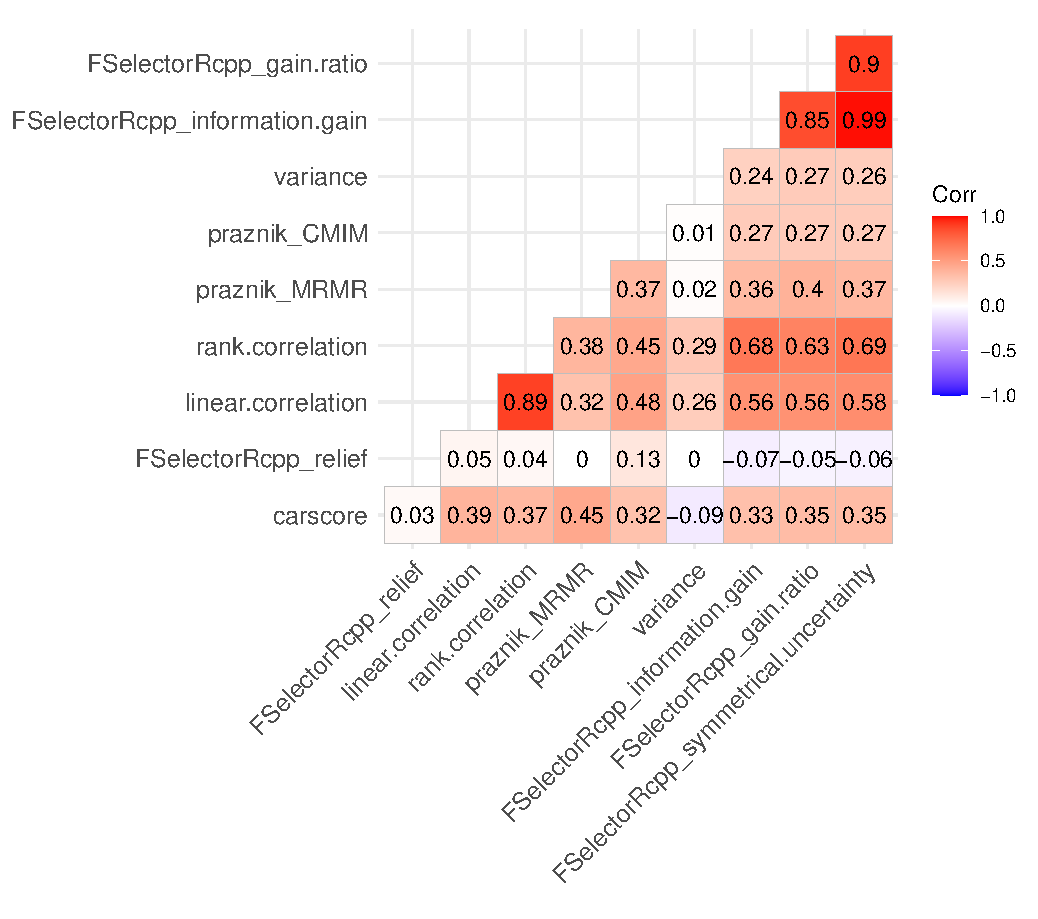
\includegraphics[width=0.7\textwidth] {correlation-filter-nri-1.pdf}
		\caption{Spearman correlations of NRI feature rankings obtained with different filters. Filter names refer to the nomenclature used by the \texttt{mlr} R package. Underscores in names divide the terminology into their upstream R package and the actual filter name.}\label{fig:correlation-filters}
	\end{center}
\end{figure}

\pagebreak

\subsection{}

\begin{table}[h!]
	\centering
	\caption[t]{Hyperparameter ranges and types for each model.
		Hyperparameter notations from the respective R packages are shown.}
	\begingroup\scriptsize
	\begin{tabularx}{.5\textwidth}{llXXrXX}
		\\
		\specialcell{Model                                              \\ (package)}                & Hyperparameter              & Type    & Start     & End      & Default \\
		\toprule
		\multirow{3}{*}{\specialcell{RF                                 \\ (ranger)}}       & \texttt{$x_{try}$}    & dbl & 0         & 0.5      & -       \\
		 & \texttt{min.node.size}      & int & 1        & 10      & 1   \\
		 & \texttt{sample.fraction}    & dbl & 0.2      & 0.9     & 1   \\
		\midrule
		\multirow{2}{*}{\specialcell{SVM                                \\ (kernlab)}}     & \texttt{C}                  & dbl & $2^{-10}$ & $2^{10}$ & 1       \\
		 & \texttt{$\sigma$}           & dbl & $2^{-5}$ & $2^{5}$ & 1   \\
		\midrule
		\multirow{7}{*}{\specialcell{XGBoost                            \\ (xgboost)}} & \texttt{nrounds}            & int & 10        & 70      & -       \\
		 & \texttt{colsample\_bytree}  & dbl & 0.6      & 1       & 1   \\
		 & \texttt{subsample}          & dbl & 0.6      & 1       & 1   \\
		 & \texttt{max\_depth}         & int & 3        & 15      & 6   \\
		 & \texttt{gamma}              & int & 0.05     & 10      & 0   \\
		 & \texttt{eta}                & dbl & 0.1      & 1       & 0.3 \\
		 & \texttt{min\_child\_weight} & int & 1        & 7       & 1   \\
		\bottomrule
	\end{tabularx}
	\endgroup
	\label{tab:hyperparameter_limits}
\end{table}

\pagebreak

\subsection{}

% \begingroup\scriptsize
% \setlength\tabcolsep{4pt}  % default value: 6pt
% vertical spacing between rows (default is 1)
{\def\arraystretch{1.7}
	\tablecaption{List of available vegetation indices in the \texttt{hsdar} package.}
	\begin{supertabular}{lll}
		% \begin{supertabular}{0.3\textwidth}{lll}
		\bfseries{Name} & \bfseries{Formula}                                                                                   & \bfseries{Reference*}         \\
		Boochs          & $D_{703}$                                                                                            & \cite{boochs1990}             \\
		Boochs2         & $D_{720}$                                                                                            & \cite{boochs1990}             \\
		CAI             & $0.5 \times (R_{2000} + R_{2200}) -R_{2100}$                                                         & \cite{nagler2003}             \\
		\midrule
		CARI            & $a = (R_{700}-R_{550}) / 150$                                                                        & \cite{walthall1994}           \\
		& $b = R_{550}-(a\times 550)$                                                                          &                               \\
		& $\frac{R_{700}\times | (a\times 670+R_{670}+b)}{R_{670}\times(a^2+1)| ^{0.5}}$                       &                               \\
		\midrule
		Carter          & $R_{695}/R_{420}$                                                                                    & \cite{carter1994}             \\
		Carter2         & $R_{695}/R_{760}$                                                                                    & \cite{carter1994}             \\
		Carter3         & $R_{605}/R_{760}$                                                                                    & \cite{carter1994}             \\
		Carter4         & $R_{710}/R_{760}$                                                                                    & \cite{carter1994}             \\
		Carter5         & $R_{695}/R_{670}$                                                                                    & \cite{carter1994}             \\
		Carter6         & $R_{550}$                                                                                            & \cite{carter1994}             \\
		CI              & $R_{675}\times R_{690}/R_{683}^2$                                                                    & \cite{zarco-tejada2003}      \\
		CI~2             & $R_{760}/R_{700}-1$                                                                                  & \cite{gitelson2003}           \\
		ClAInt          & $\int_{600 nm}^{735 nm} R$                                                                           & \cite{oppelt2004}             \\
		CRI1            & $1/R_{515}-1/R_{550}$                                                                                & \cite{gitelson2003}           \\
		CRI2            & $1/R_{515}-1/R_{770}$                                                                                & \cite{gitelson2003}           \\
		CRI3            & $1/R_{515}-1/R_{550}\times R_{770}$                                                                  & \cite{gitelson2003}           \\
		CRI4            & $1/R_{515}-1/R_{700}\times R_{770}$                                                                  & \cite{gitelson2003}           \\
		D1              & $D_{730}/D_{706}$                                                                                    & \cite{zarco-tejada2003}      \\
		D2              & $D_{705}/D_{722}$                                                                                    & \cite{zarco-tejada2003}      \\
		Datt            & $(R_{850}-R_{710})/(R_{850}-R_{680})$                                                                & \cite{datt1999}               \\
		Datt2           & $R_{850}/R_{710}$                                                                                    & \cite{datt1999}               \\
		Datt3           & $D_{754}/D_{704}$                                                                                    & \cite{datt1999}               \\
		Datt4           & $R_{672}/(R_{550} \times R_{708})$                                                                   & \cite{datt1998}               \\
		Datt5           & $R_{672}/R_{550}$                                                                                    & \cite{datt1998}               \\
		Datt6           & $(R_{860})/(R_{550}\times R_{708})$                                                                  & \cite{datt1998}               \\
		Datt7           & $(R_{860} - R_{2218})/(R_{860} - R_{1928})$                                                          & \cite{datt1999a}              \\
		Datt8           & $(R_{860} - R_{1788})/(R_{860} - R_{1928})$                                                          & \cite{datt1999a}              \\
		DD              & $(R_{749}-R_{720})-(R_{701}-R_{672})$                                                                & \cite{maire2004}              \\
		DDn             & $2\times (R_{710}-R_{660}-R_{760})$                                                                  & \cite{lemaire2008}            \\
		DPI             & $(D_{688}*D_{710})/D_{697}^2$                                                                        & \cite{zarco-tejada2003}      \\
		DWSI1           & $R_{80}/R_{1660}$                                                                                    & \cite{apan2004}               \\
		DWSI2           & $R_{1660}/R_{550}$                                                                                   & \cite{apan2004}               \\
		DWSI3           & $R_{1660}/R_{680}$                                                                                   & \cite{apan2004}               \\
		DWSI4           & $R_{550}/R_{680}$                                                                                    & \cite{apan2004}               \\
		DWSI5           & $(R_{800} + R_{550})/(R_{1660} + R_{680})$                                                           & \cite{apan2004}               \\
		EGFN            & $\frac{(\max(D_{650:750})-\max(D_{500:550}))}{(\max(D_{650:750})+\max(D_{500:550}))}$                & \cite{penuelas1994}           \\
		EGFR            & $\max(D_{650:750})/\max(D_{500:550})$                                                                & \cite{penuelas1994}           \\
		EVI             & $\frac{2.5\times ((R_{800}-R_{670}) }{ (R_{800}-(6\times R_{670})-(7.5\times R_{475})+1)}$           & \cite{huete1997}             \\
		GDVI            & $(R_{800}^n-R_{680}^n) / (R_{800}^n+R_{680}^n)$**                                                    & \cite{wu2014}                 \\
		GI              & $R_{554}/R_{677}$                                                                                    & \cite{smith1995}              \\
		Gitelson        & $1/R_{700}$                                                                                          & \cite{gitelson1999}           \\
		Gitelson2       & $(R_{750}-R_{800}/R_{695}-R_{740})-1$                                                                & \cite{gitelson2003}           \\
		GMI1            & $R_{750}/R_{550}$                                                                                    & \cite{gitelson2003}           \\
		GMI2            & $R_{750}/R_{700}$                                                                                    & \cite{gitelson2003}           \\
		Green NDVI      & $\frac{R_{800}-R_{550}}{R_{800}+R_{550}}$                                                            & \cite{gitelson1996}           \\
		LWVI\_1         & $\frac{(R_{1094}-R_{983})}{(R_{1094}+R_{983})}$                                                      & \cite{galvao2005}             \\
		LWVI\_2         & $\frac{R_{1094}-R_{1205}}{R_{1094}+R_{1205}}$                                                        & \cite{galvao2005}             \\
		Maccioni        & $\frac{R_{780}-R_{710})}{R_{780}-R_{680}}$                                                           & \cite{maccioni2001}           \\
		\midrule
		MCARI           & \parbox{5.5cm}{$((R_{700}-R_{670})-0.2\times (R_{700}-R_{550})) \times (R_{700}/R_{670})$}           & \cite{daughtry2000}           \\
		\midrule
		MCARI2          & \parbox{5.5cm}{$((R_{750}-R_{705})-0.2 \times (R_{750}-R_{550})) \times (R_{750}/R_{705})$}          & \cite{wu2008}                \\
		\midrule
		mND705          & $\frac{(R_{750}-R_{705})}{R_{750}+R_{705}-2\times R_{445}}$                                          & \cite{sims2002}              \\
		mNDVI           & $\frac{(R_{800}-R_{680})}{R_{800}+R_{680}-2 \times R_{445}}$                                         & \cite{sims2002}              \\
		MPRI            & $\frac{R_{515}-R_{530}}{R_{515}+R_{530}}$                                                            & \cite{hernandez-clemente2011} \\
		MSAVI           & \parbox{5.5cm}{$0.5 \times ((2\times R_{800}+1)^2-8\times (R_{800}-R_{670}))^{0.5}$}                 & \cite{qi1994}                 \\
		MSI             & $\frac{R_{1600}}{R_{817}}$                                                                           & \cite{hunt1989}               \\
		mSR             & $\frac{R_{800}-R_{445}}{R_{680}-R_{445}}$                                                            & \cite{sims2002}              \\
		mSR2            & $\frac{(R_{750}/R_{705})-1}{R_{750}/R_{705}+1)^{0.5}}$                                               & \cite{chen1996}               \\
		mSR705          & $\frac{R_{750}-R_{445}}{R_{705}-R_{445}}$                                                            & \cite{sims2002}              \\
		MTCI            & $\frac{R_{754}-R_{709}}{R_{709}-R_{681}}$                                                            & \cite{dash2007}               \\
		\midrule
		MTVI            & \parbox{3.8cm}{$1.2 \times (1.2 \times (R_{800}-R_{550})-2.5 \times (R_{670}-R_{550}))$}             & \cite{haboudane2002}          \\
		\midrule
		NDLI            & $\frac{log(1/R_{1754}) - log(1/R_{1680})}{log(1/R_{1754}) + log(1/R_{1680})}$                        & \cite{serrano2002}            \\
		NDNI            & $\frac{log(1/R_{1510}) - log(1/R_{1680})}{log(1/R_{1510}) + log(1/R_{1680})}$                        & \cite{serrano2002}            \\
		NDVI            & $\frac{R_{800}-R_{680}}{R_{800}+R_{680}}$                                                            & \cite{tucker1979}             \\
		NDVI2           & $\frac{R_{750}-R_{705}}{R_{750}+R_{705}}$                                                            & \cite{gitelson1994}           \\
		NDVI3           & $\frac{R_{682}-R_{553}}{R_{682}+R_{553}}$                                                            & \cite{guanter2005}            \\
		NDWI            & $\frac{R_{860}-R_{1240}}{R_{860}+R_{1240}}$                                                          & \cite{gao1996}                \\
		NPCI            & $\frac{R_{680}-R_{430}}{R_{680}+R_{430}}$                                                            & \cite{penuelas1994}           \\
		OSAVI           & $\frac{(1+0.16) \times (R_{800}-R_{670})}{R_{800}+R_{670}+0.16 }$                                    & \cite{rondeaux1996}           \\
		OSAVI2          & $\frac{(1+0.16)\times (R_{750}-R_{705})}{R_{750}+R_{705}+0.16) }$                                    & \cite{wu2008}                \\
		PARS            & $\frac{R_{746}}{R_{513}}$                                                                            & \cite{chappelle1992}          \\
		PRI             & $\frac{R_{531}-R_{570}}{R_{531}+R_{570}}$                                                            & \cite{gamon1992}              \\
		PRI\_norm       & $\frac{PRI \times (-1) }{RDVI\times R_{700}/R_{670}}$                                                & \cite{zarco-tejada2013}      \\
		PRI*CI2         & $PRI*CI2$                                                                                            & \cite{garrity2011}            \\
		PSRI            & $\frac{R_{678}-R_{500}}{R_{750}}$                                                                    & \cite{merzlyak1999}           \\
		PSSR            & $\frac{R_{800}}{R_{635}}$                                                                            & \cite{blackburn1998}          \\
		PSND            & $\frac{R_{800}-R_{470}}{R_{800}-R_{470})}$                                                           & \cite{blackburn1998}          \\
		PWI             & $\frac{R_{900}}{R_{970}}$                                                                            & \cite{penuelas1997}           \\
		RDVI            & $\frac{R_{800}-R_{670}}{ \sqrt{R_{800}+R_{670}}}$                                                    & \cite{roujean1995}            \\
		\midrule
		REP\_LE         & \parbox{3.8cm}{Red-edge position through linear extrapolation}                                       & \cite{cho2006}                \\
		\midrule
		REP\_Li         & $R_{re}=\frac{R_{670}+R_{780})}{2}$                                                                  & \cite{guyot1988}              \\
		& $\frac{700 + 40 \times ((R_{re} -R_{700})}{(R_{740}-R_{700}))}$                                      &                               \\
		\midrule
		SAVI            & $\frac{(1+L)\times (R_{800}-R_{670})}{(R_{800}+R_{670}+L)}$                                          & \cite{huete1988}              \\
		SIPI            & $\frac{R_{800}-R_{445}}{R_{800}-R_{680}}$                                                            & \cite{penuelasj.1995}         \\
		\midrule
		SPVI            & \parbox{3.8cm}{$0.4 \times 3.7 \times (R_{800}-R_{670})-1.2 \times ((R_{530}-R_{670})^2)^{0.5}$}     & \cite{vincini2006}            \\
		\midrule
		SR              & $\frac{R_{800}}{R_{680}}$                                                                            & \cite{jordan1969}             \\
		SR1             & $\frac{R_{750}}{R_{700}}$                                                                            & \cite{gitelson1997}           \\
		SR2             & $\frac{R_{752}}{R_{690}}$                                                                            & \cite{gitelson1997}           \\
		SR3             & $\frac{R_{750}}{R_{550}}$                                                                            & \cite{gitelson1997}           \\
		SR4             & $\frac{R_{700}}{R_{670}}$                                                                            & \cite{mcmurtrey1994}          \\
		SR5             & $\frac{R_{675}}{R_{700}}$                                                                            & \cite{chappelle1992}          \\
		SR6             & $\frac{R_{750}}{R_{710}}$                                                                            & \cite{zarco-tejada1999}       \\
		SR7             & $\frac{R_{440}}{R_{690}}$                                                                            & \cite{lichtenthaler1996}      \\
		SR8             & $\frac{R_{515}}{R_{550}}$                                                                            & \cite{hernandez-clemente2012} \\
		SRPI            & $\frac{R_{430}}{R_{680}}$                                                                            & \cite{penuelasj.1995}         \\
		SRWI            & $\frac{R_{850}}{R_{1240}}$                                                                           & \cite{zarco-tejada2003}      \\
		Sum\_Dr1        & $\sum_{i=626}^{795} D1_i$                                                                            & \cite{elvidge1995}            \\
		Sum\_Dr2        & $\sum_{i=680}^{780} D1_i$                                                                            & \cite{filella1994}            \\
		SWIR FI         & $\frac{R_{2133}^2}{R_{2225} \times R_{2209}^3}$                                                      & \cite{levin2007}              \\
		\midrule
		SWIR LI         & \parbox{3.8cm}{$3.87  \times (R_{2210} - R_{2090}) - 27.51 \times (R_{2280} - R_{2090}) - 0.2$}      & \cite{lobell2001}             \\
		\midrule
		SWIR SI         & \parbox{3.8cm}{$-41.59 \times (R_{2210} - R_{2090}) + 1.24 \times (R_{2280} - R_{2090}) + 0.64 $}    & \cite{lobell2001}             \\
		\midrule
		SWIR VI         & \parbox{3.8cm}{$37.72  \times (R_{2210} - R_{2090}) + 6.27 \times (R_{2280} - R_{2090}) + 0.57$}     & \cite{lobell2001}             \\
		\midrule
		TCARI           & \parbox{3.8cm}{$3*((R_{700}-R_{670})-0.2\times R_{700}-R_{550})\times (R_{700}/R_{670}))$}           & \cite{haboudane2002}          \\
		\midrule
		TCARI/OSAVI     & TCARI/OSAVI                                                                                          & \cite{haboudane2002}          \\
		\midrule
		TCARI2          & \parbox{3.8cm}{$3 \times ((R_{750}-R_{705})-0.2 \times (R_{750}-R_{550}) \times (R_{750}/R_{705}))$} & \cite{wu2008}                \\
		\midrule
		TCARI2/OSAVI2   & TCARI2/OSAVI2                                                                                        & \cite{wu2008}                \\
		\midrule
		TGI             & \parbox{3.8cm}{$-0.5 (190 (R_{670} - R_{550} ) - 120 (R_{670} - R_{480}))$}                          & \cite{hunt2013}               \\
		\midrule
		TVI             & \parbox{3.8cm}{$0.5\times (120 \times (R_{750}-R_{550})-200 \times (R_{670}-R_{550}))$}              & \cite{broge2001}              \\
		\midrule
		Vogelmann       & $\frac{R_{740}}{R_{720}}$                                                                            & \cite{vogelmann1993}          \\
		Vogelmann2      & $\frac{R_{734}-R_{747}}{R_{715}+R_{726})}$                                                           & \cite{vogelmann1993}          \\
		Vogelmann3      & $\frac{D_{715}}{D_{705}}$                                                                            & \cite{vogelmann1993}          \\
		Vogelmann4      & $\frac{R_{734}-R_{747}}{R_{715}+R_{720}}$                                                            & \cite{vogelmann1993}     \\
	\end{supertabular}
	\label{tab:vegindices}
}

\pagebreak

\subsection{}

The following information was provided by the Institut Carogràfic i Geològic de Catalunya, which was in charge of image acquisition and data preprocessing.

The AISA EAGLE-II sensor was used for airborne image acquisition with a field of view of 37.7~°.
Its spectral resolution is 2.4~nm and ranged from 400~nm\ to 1000~nm.

The conversion of Digital Numbers (DN) to spectral radiance was made by using software designed for the instrument.
Images were originally scaled in 12 bits but were radiometrically calibrated to 16 bits, reserving the highest value (65535) for null values.
The procedure was applied to the 23 previously selected images.
Last, the geometric and atmospheric corrections were applied to the images.

The aim of this procedure was to reduce the positional errors of the images.
The cartographic reference system in use was EPSG~25830.
Positioning was done by coupling an Applanix POS AV 410 system to the sensor, integrating GPS and IMU systems.
The system provides geographic coordinates of the terrain and relative coordinates of the aircraft (attitude) at each scanned line.
Additionally a DSM from GeoEuskadi with a spatial resolution of 1~m was used.
The ortorectified hyperspectral images were compared to orthoimages (1:5000) from GeoEuskadi.
This comparison was used as the base to calculate RMSE, which was below the ground sampling distance in the across and along track directions.

The radiance measured by an instrument depends on the illumination geometry and the reflective properties of the observed surface.
Radiation may be absorbed or scattered (Rayleigh and Mie scattering).
Scattering is responsible for the adjacency effect, i.e., radiation coming from neighbors' areas to the target pixel.
The MODTRAN algorithm was used to model the effect of the atmosphere on the radiation.
To represent the aerosols of the study area, the rural model was used.
In addition the optical thickness was estimated on pixels with a high vegetation cover.
Columnar water vapor was estimated by a linear regression ratio where the spectral radiance of each pixel at the band of the maximum water absorption (~906~nm) is compared to its theoretical value in the\ absence of absorption.
Nonetheless, this technique is unreliable in the\ presence of a spectral resolution as in this case.
To resolve this, the water vapor parameter was selected manually according to the smoothness observed on the reflectance peak at 960~nm.
This was combined with a mid-latitude summer atmosphere model.
The output of this procedure was reflectance from the target pixel scaled between 0 and 10,000.

The image acquisitions were originally attempted during one day (29.10.2016).
Due to the variable meteorological conditions, some stands had to be imaged one day later.

%%%%%%%%%%%%%%%%%%%%%%%%%%%%%%%%%%%%%%%%%%
\end{paracol}
%%%%%%%%%%%%%%%%%%%%%%%%%%%%%%%%%%%%%%%%%%
% To add notes in main text, please use \endnote{} and un-comment the codes below.
%\begin{adjustwidth}{-5.0cm}{0cm}
%\printendnotes[custom]
%\end{adjustwidth}
%%%%%%%%%%%%%%%%%%%%%%%%%%%%%%%%%%%%%%%%%%
\reftitle{References}

% Please provide either the correct journal abbreviation (e.g. according to the “List of Title Word Abbreviations” http://www.issn.org/services/online-services/access-to-the-ltwa/) or the full name of the journal.
% Citations and References in Supplementary files are permitted provided that they also appear in the reference list here.

%=====================================
% References, variant A: external bibliography
%=====================================
\externalbibliography{yes}
\bibliography{Biblio}

% If authors have biography, please use the format below
\section*{Short Biography of Authors}
\bio
{\raisebox{-0.35cm}{
\includegraphics[width=3.5cm,height=5.3cm,clip,keepaspectratio]{pschratz.jpeg}}}
{\textbf{Patrick Schratz} is a Data Scientist working in Zurich, Switzerland.
	His area of expertise is applied machine learning, more specifically the field of environmental modeling.
	He is a Ph.D. candidate in geographic information science in the Department of Geography at Friedrich Schiller University Jena where he conducts research in environmental modeling.
	At cynkra GmbH in Zurich, Patrick is an R consultant with many years of experience in the following fields: CI/CD, package development, DevOps tasks, machine learning and spatiotemporal data handling.}

\bio
{\raisebox{-0.35cm}{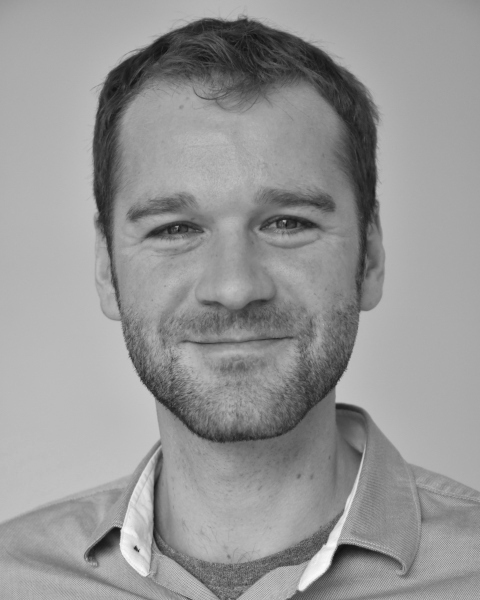
\includegraphics[width=3.5cm,height=5.3cm,clip,keepaspectratio]{jmuenchow.jpg}}}
{\textbf{Jannes Muenchow} is a GIScientist working in tropical ecology since 2007 with a special interest in ENSO, biodiversity, species distribution modeling and predictive mapping.
	He received his Ph.D. from Friedrich-Alexander-Universität Erlangen-Nürnberg (Germany) in 2013.
	He joined the business location department of a large consulting company as a geo-data scientist for more than two years until the prediction of a strong El Niño event brought him back to academia from 2016 to 2019 (Friedrich Schiller University Jena).
	His research focuses on developing open-source tools for ecology, geomorphology and qualitative GIS.
	He is a co-author of the book ``Geocomputation with R''.}

\bio
{\raisebox{-0.35cm}{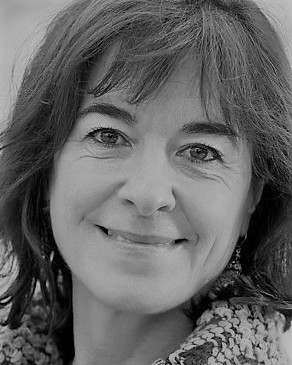
\includegraphics[width=3.5cm,height=5.3cm,clip,keepaspectratio]{eiturritxa.jpg}}}
{\textbf{Eugenia Iturritxa} received the Ecology and Ph.D. degree in Plant Protection from the University of the Basque Country in 2001.
	Since 1999 her main research has focused on forest health, on the study of diverse species of native and introduced pathogenic fungi in forests and forest plantations.
	Her research the NEIKER research center includes the distribution of diseases, analysis of predisposing factors for them, genetic and phenotypic studies of populations and their epidemiology.}

\bio
{\raisebox{-0.35cm}{
\includegraphics[width=3.5cm,height=5.3cm,clip,keepaspectratio]{jcortes.png}}}
{\textbf{José Cortés} received his B.S. in Mathematics and M.S. in Statistics from Arizona State University, Arizona, USA, in 2014 and 2016, respectively.
	Currently he is a Ph.D. student at Friedrich Schiller University Jena, Germany.
	He is a member of the International Max Planck Research School on Global Biogeochemical Cycles (IMPRS-gBGC), a joint program with the Max Planck Institute for Biogeochemistry.
	His research focuses on spatiotemporal trend detection in environmental data.}

\bio
{\raisebox{-0.35cm}{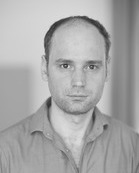
\includegraphics[width=3.5cm,height=5.3cm,clip,keepaspectratio]{bbischl.jpg}}}
{\textbf{Bernd Bischl} obtained his Ph.D. from TU Dortmund University in 2013.
	He is a professor of Statistical Learning and Data Science in the Department of Statistics at Ludwig-Maximilians-Universität in Munich, Germany, and a director of the Munich Center for Machine Learning.
	His research interests include AutoML, model selection, interpretable ML and XAI.}

\bio
{\raisebox{-0.35cm}{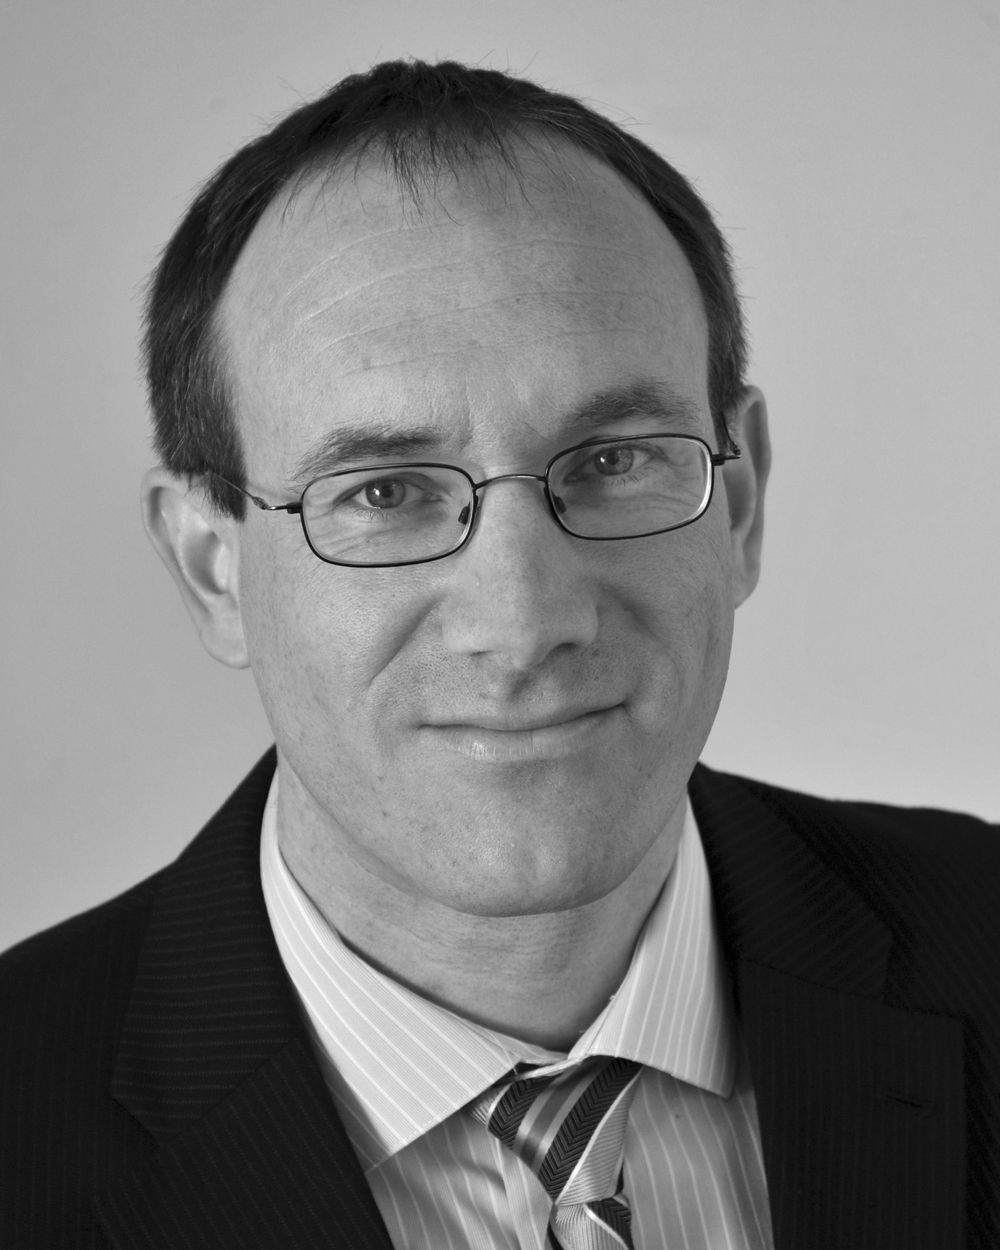
\includegraphics[width=3.5cm,height=5.3cm,clip,keepaspectratio]{abrenning.jpg}}}
{\textbf{Alexander Brenning} (Ph.D.~2005) graduated in mathematics at Technical University of Freiberg, Germany, and received his Ph.D. in geography from Humboldt-Universität zu~Berlin.
	He served as an assistant professor and tenured associate professor in geomatics at the University of Waterloo, Ontario, Canada from 2007 until 2015, when he was appointed as a full professor in geographic information science at Friedrich Schiller University Jena, Germany.
	Dr.~Brenning's research interests include statistical and machine-learning techniques for environmental modeling and remote sensing.
	He has also contributed to open-source geocomputation by developing R packages for spatial cross-validation and GIS coupling.}

%%%%%%%%%%%%%%%%%%%%%%%%%%%%%%%%%%%%%%%%%%
%% for journal Sci
%\reviewreports{\\
%Reviewer 1 comments and authors’ response\\
%Reviewer 2 comments and authors’ response\\
%Reviewer 3 comments and authors’ response
%}
%%%%%%%%%%%%%%%%%%%%%%%%%%%%%%%%%%%%%%%%%%
\end{document}

